\subsubsection{Software testing and devops practices used (D3)}
\label{testing_practices}
% 
% Testing is an important process in improving the quality of the software
% product. The purpose of this process is to find errors, which might occur during
% specification, design, and coding phases. We report the following results next:
We asked five questions to determine the adoption of testing and devops techniques in the Bangladesh software companies:
\begin{inparaenum}
\item Software Testing Practices (Q14),
\item Level of Automated Testing (Q15),
\item Tools Used in Testing and QA (Q16),
\item Continuous Deployment tools (Q17), and
\item Version Control (Q18).
\end{inparaenum}

\begin{figure}[t]
    \centering
    \caption{Software testing and devops practices used by the respondents}
    \begin{subfigure}{0.5\textwidth}
        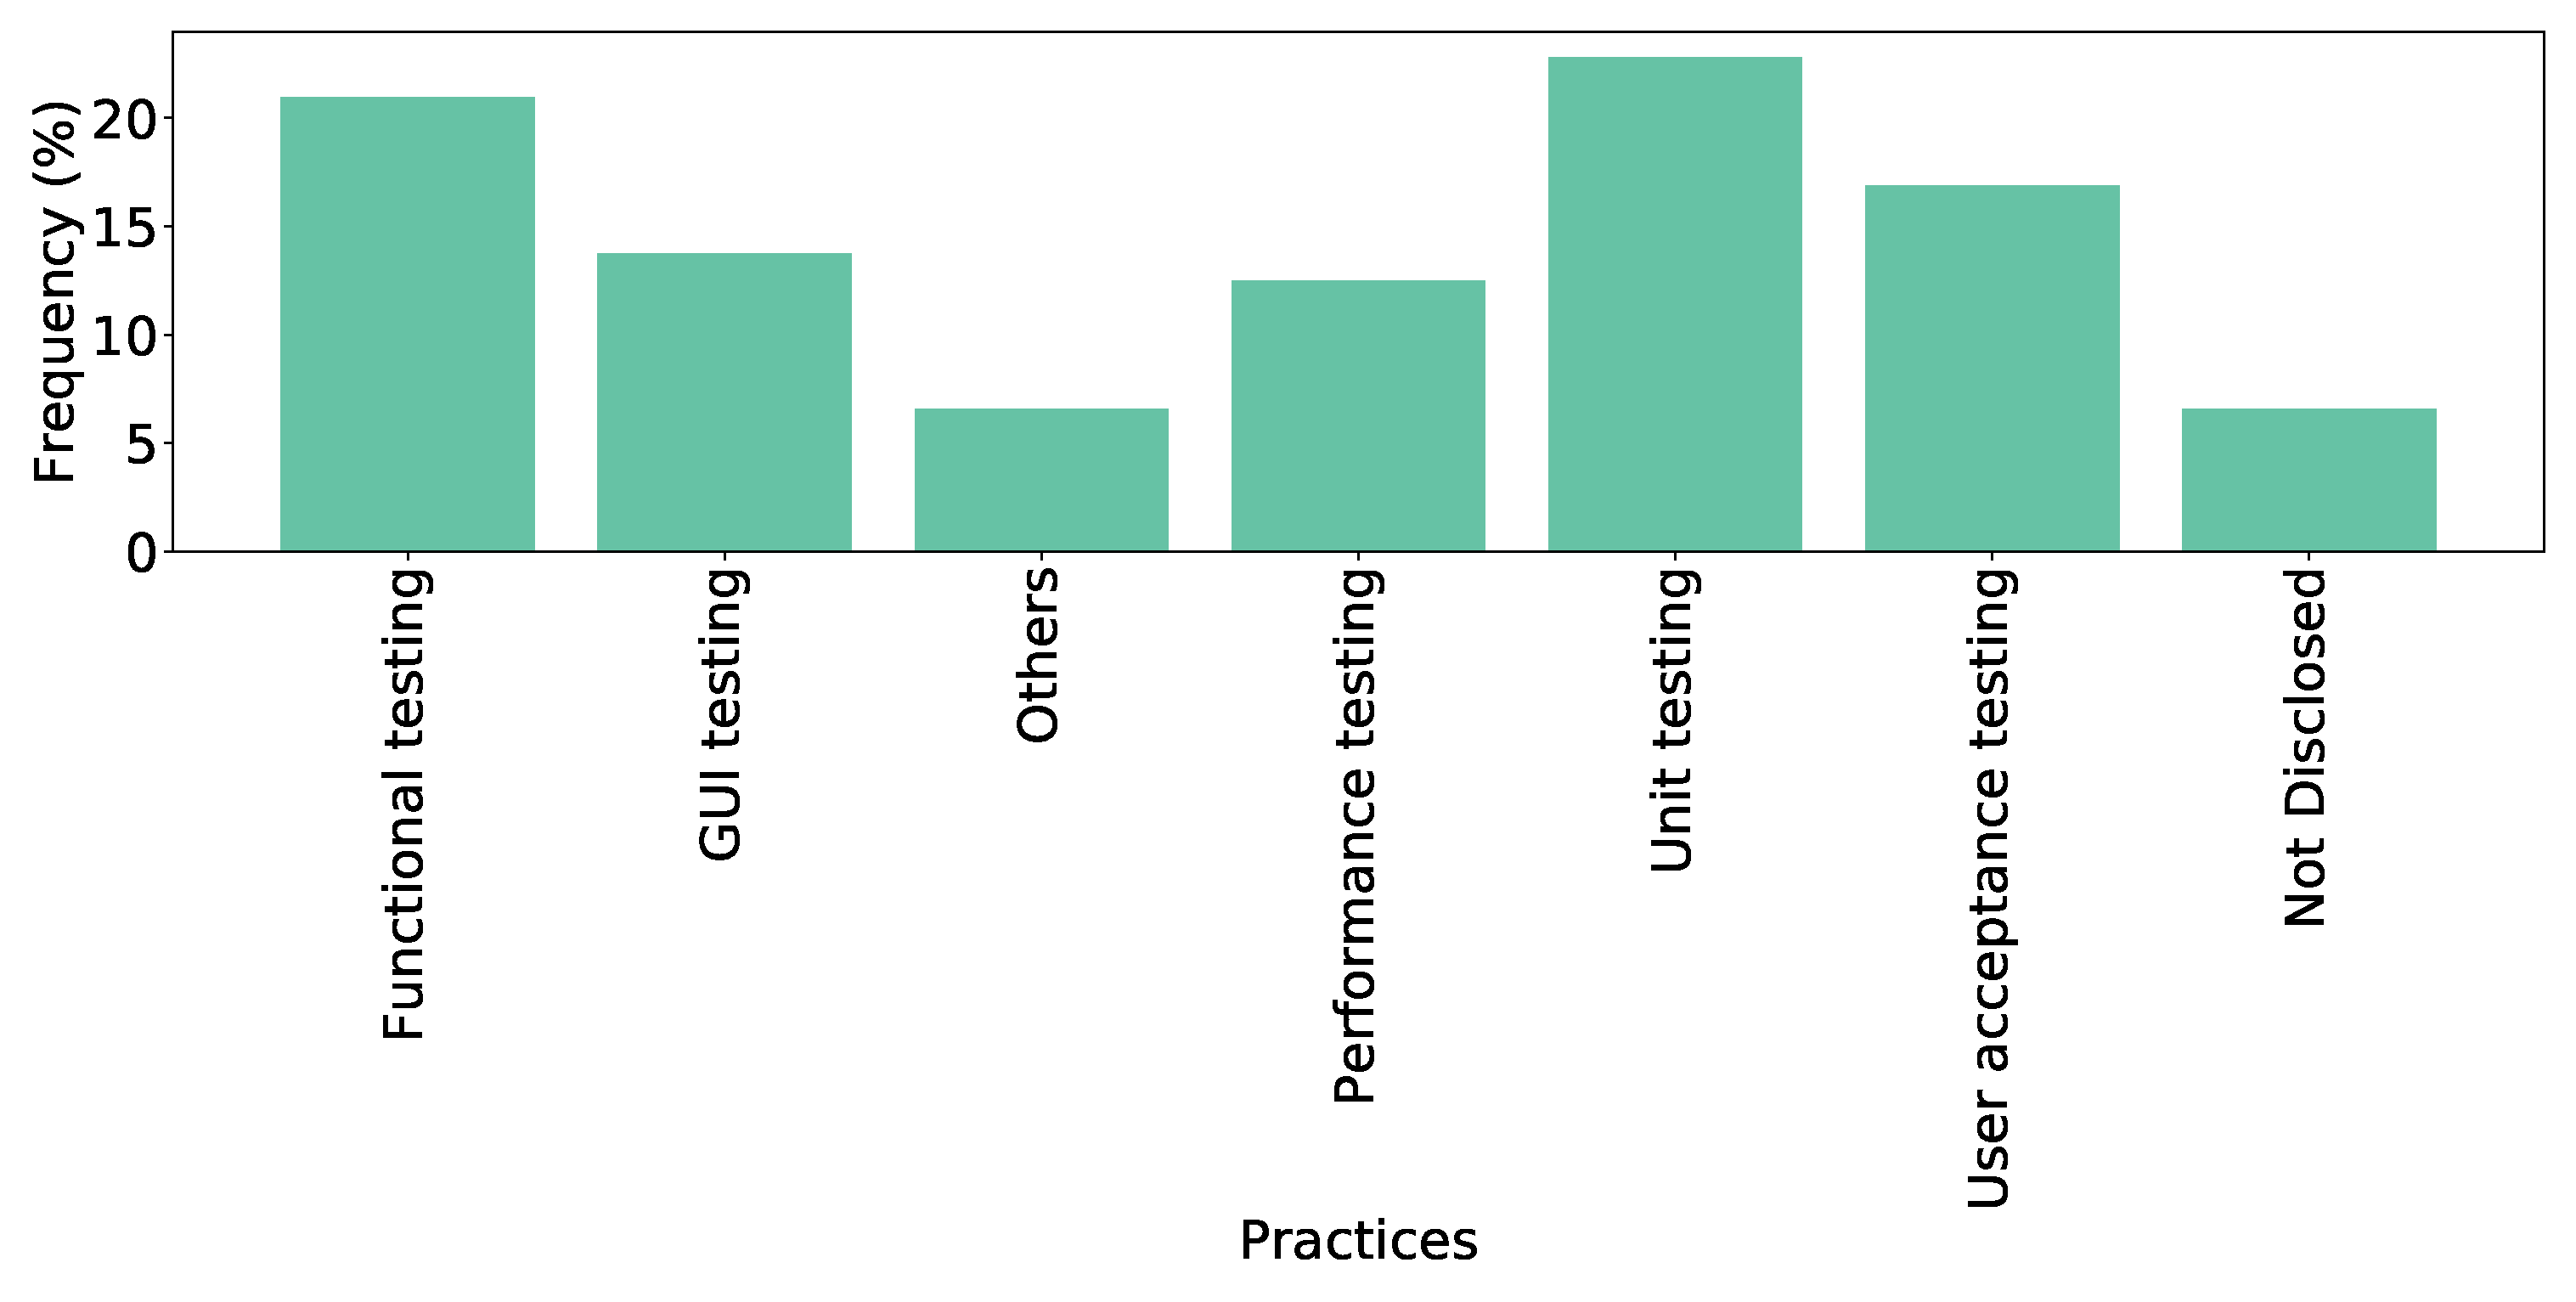
\includegraphics[scale=0.1]{Figures/Respondents_testing_practices}
        \caption{Software Testing Practices (Q14)}
        \label{fig:testing}
    \end{subfigure}
    \begin{subfigure}{0.4\textwidth}
        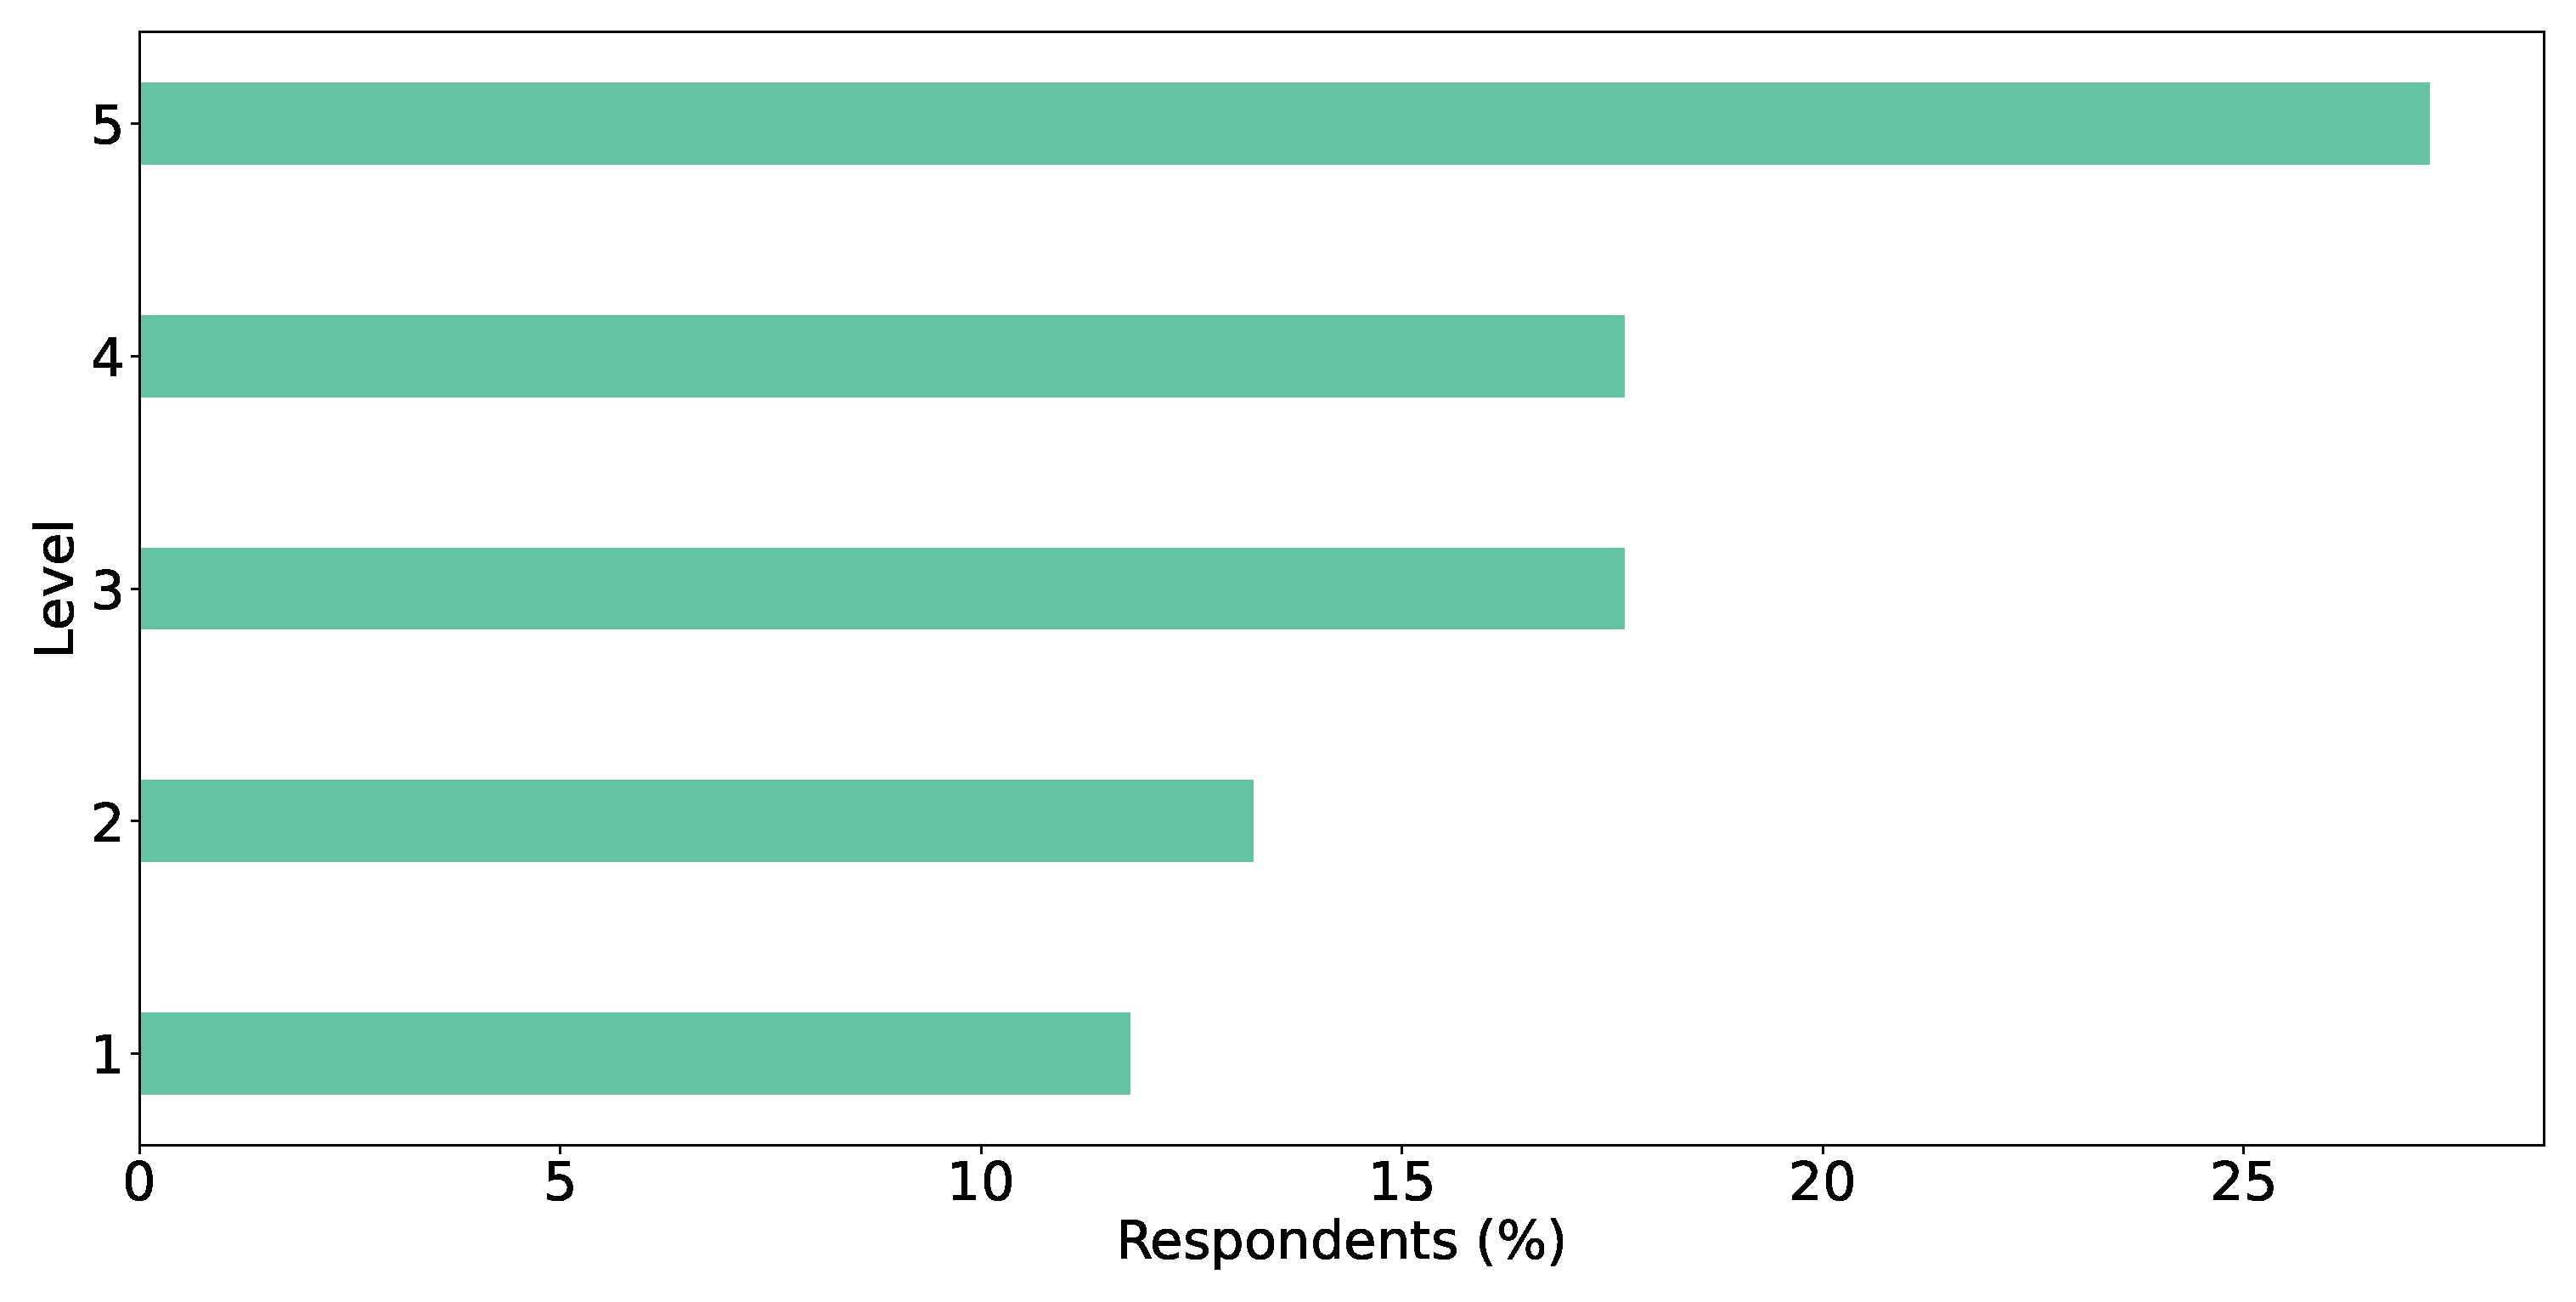
\includegraphics[scale=0.09]{Figures/Respondents_autotest_level}
        \caption{Level of Automated Testing (Q15)}
        \label{fig:autoTest}
    \end{subfigure}
    \begin{subfigure}{0.45\textwidth}
        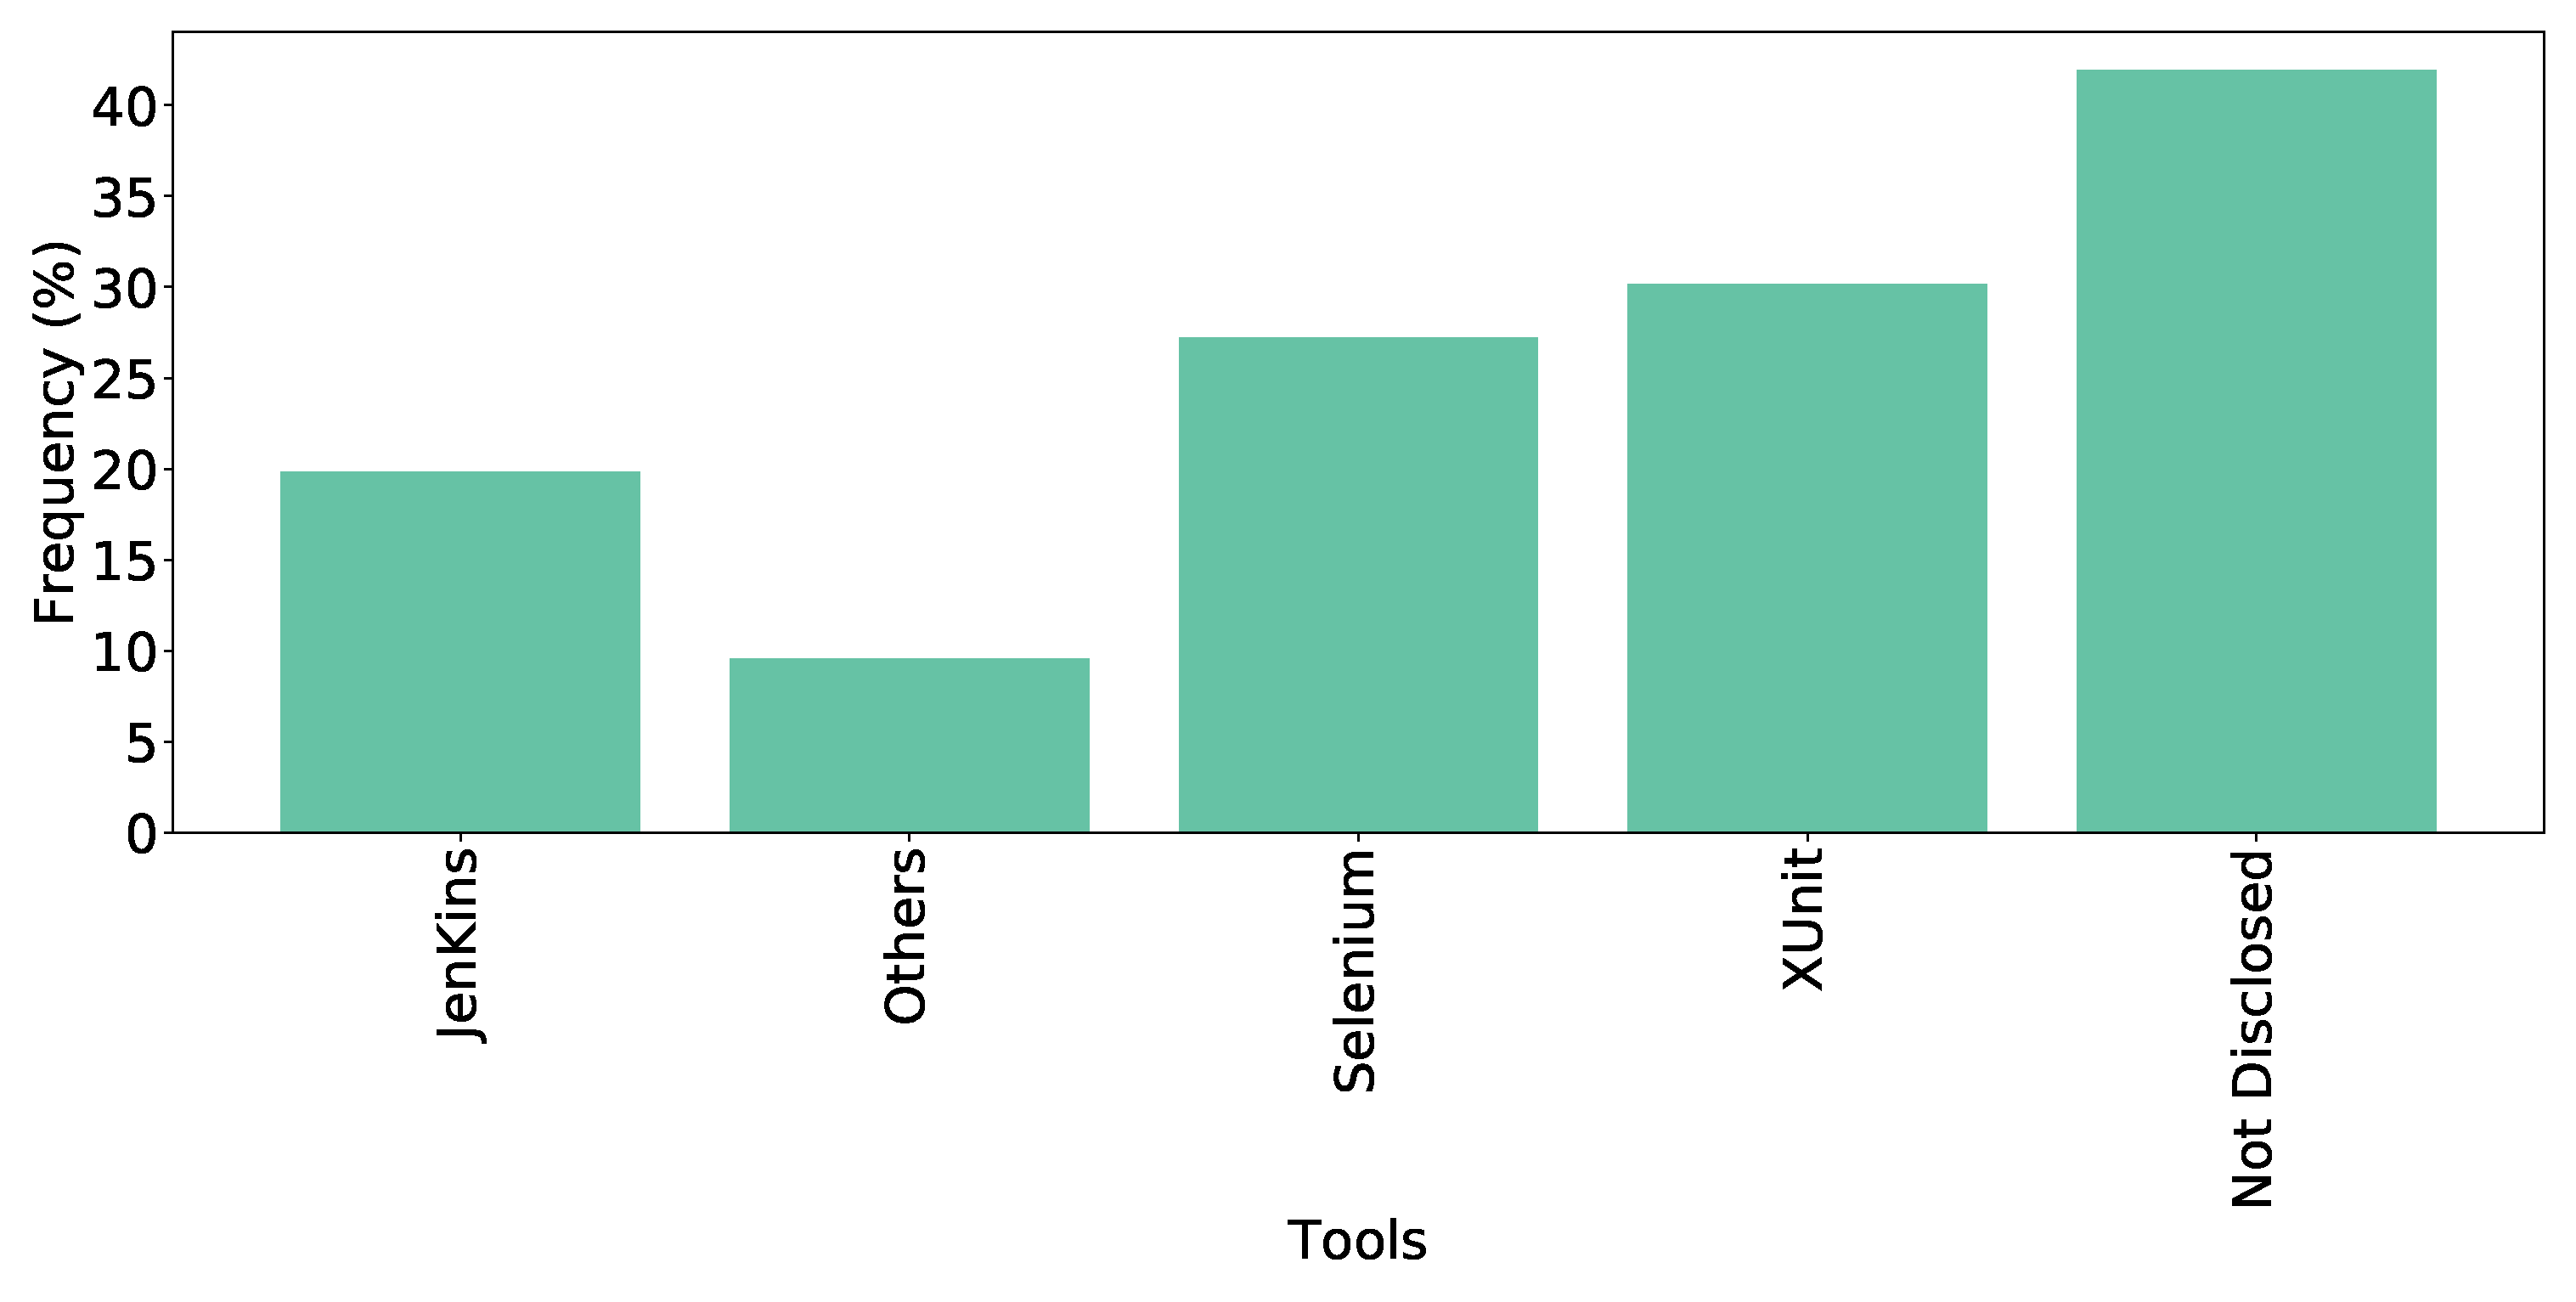
\includegraphics[scale=0.1]{Figures/Respondents_testing_tools}
        \caption{Tools Used in Testing and QA (Q16)}
        \label{fig:testingTools}
    \end{subfigure}
    \begin{subfigure}{0.45\textwidth}
        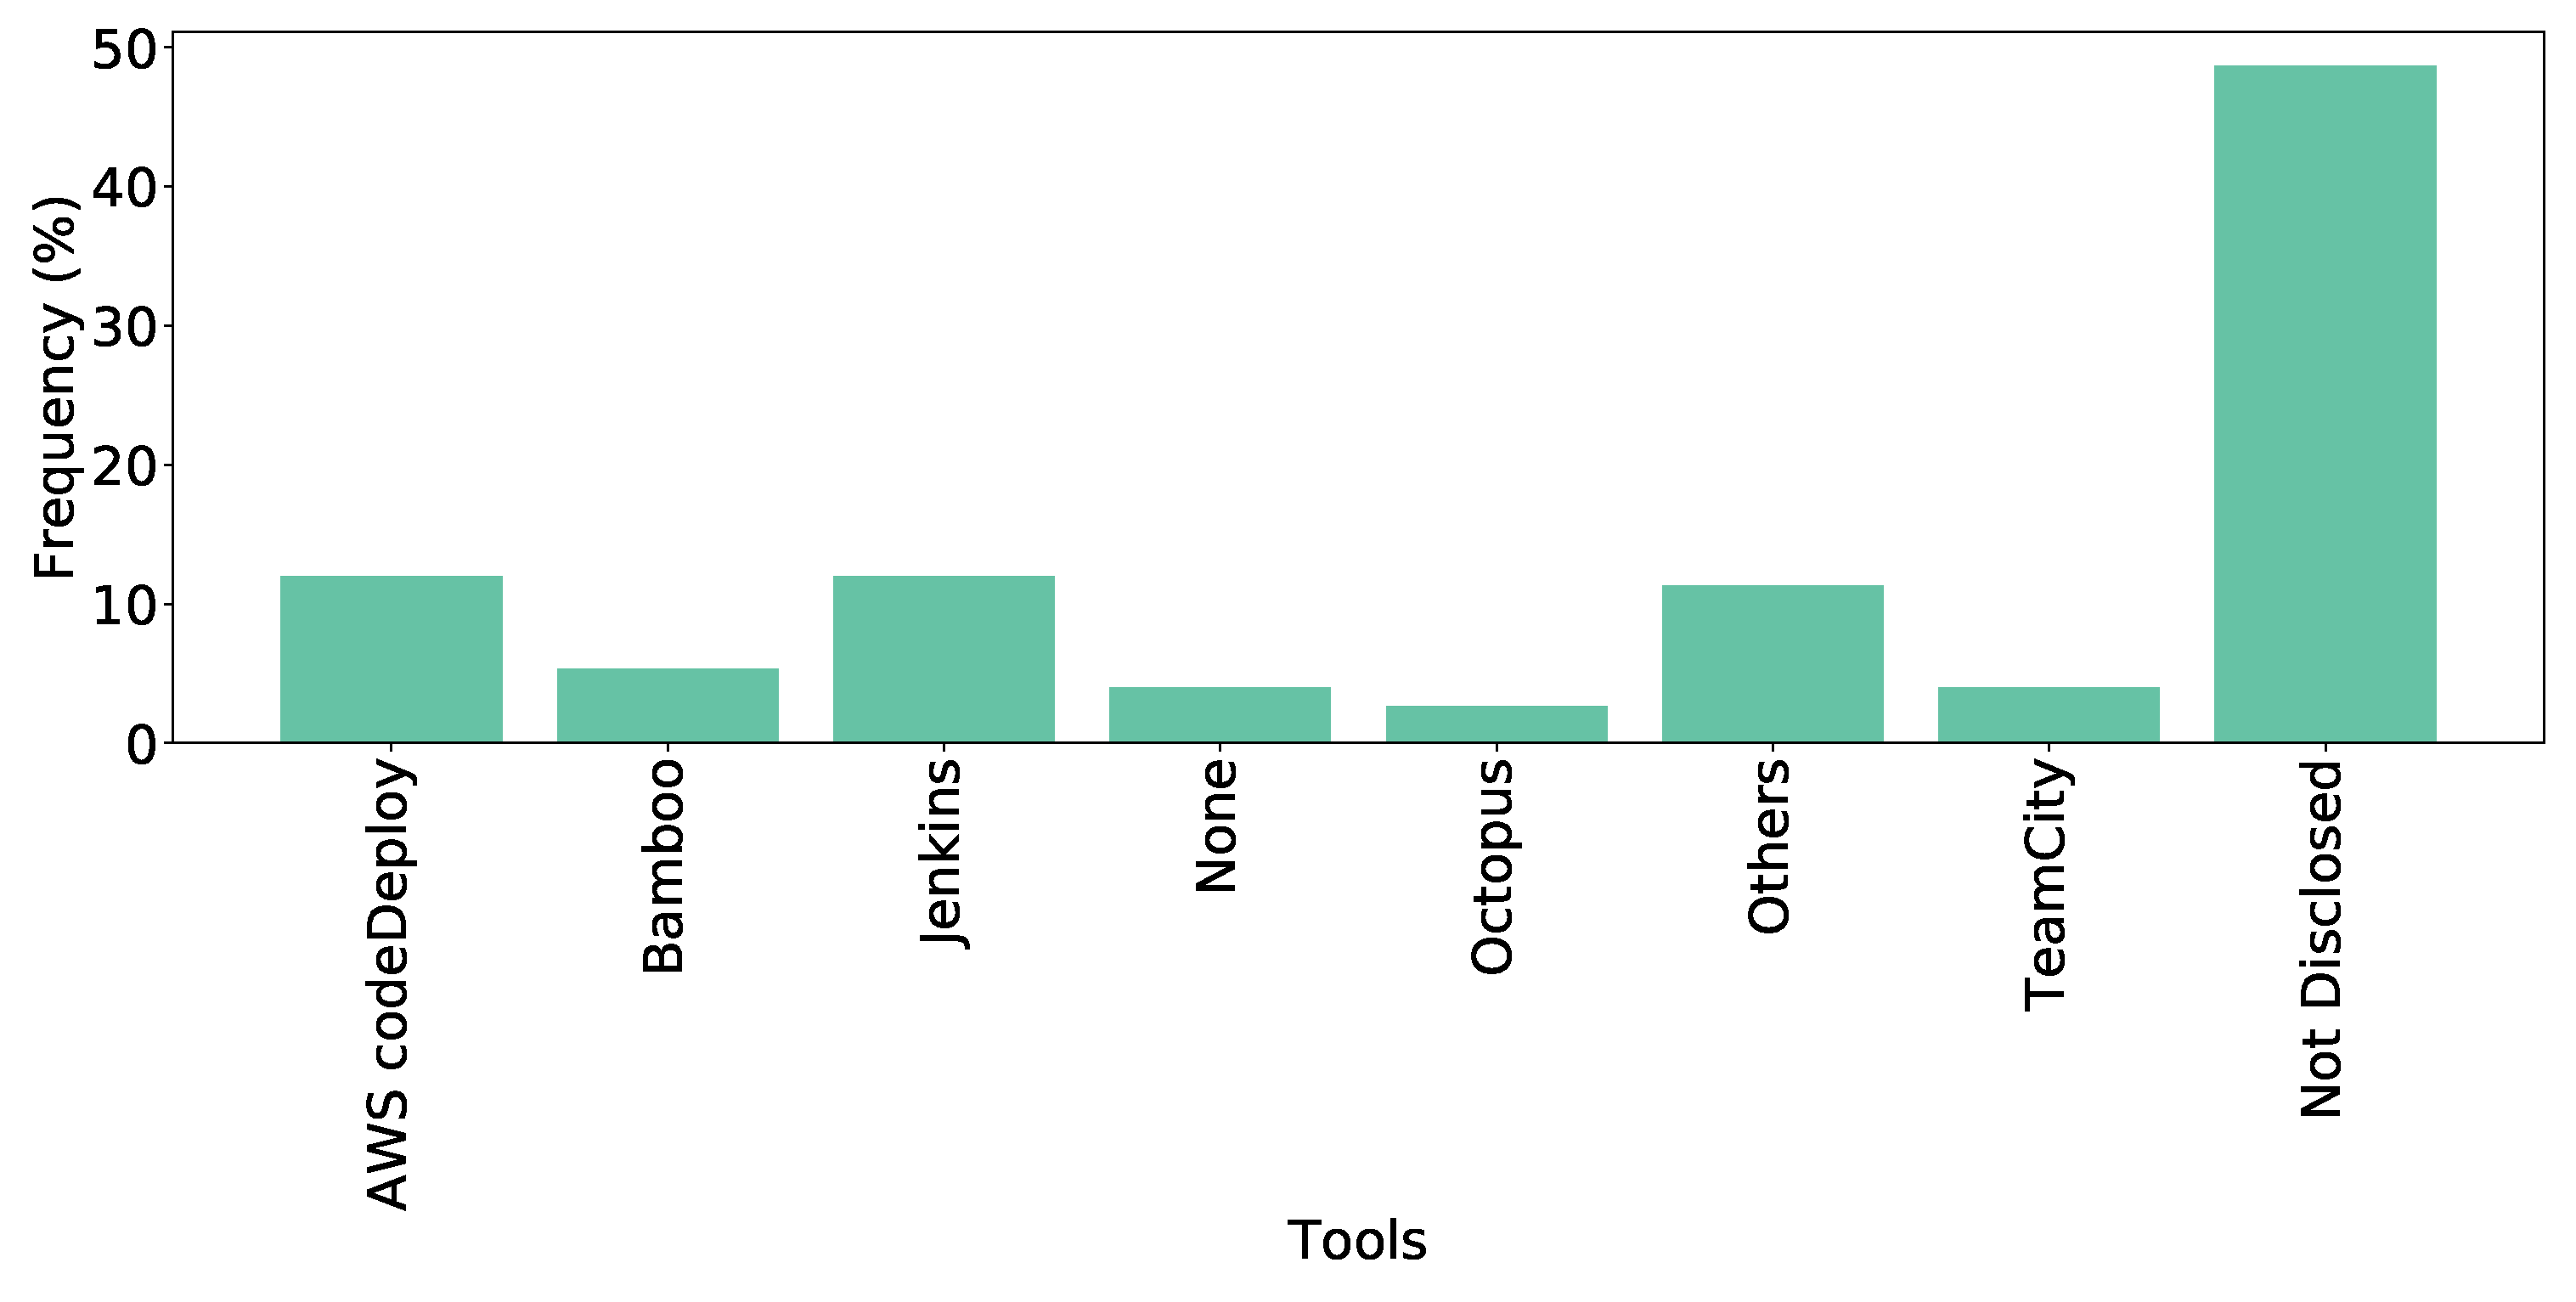
\includegraphics[scale=0.1]{Figures/Respondents_deployment_tools}
        \caption{Continuous Deployment tools (Q17)}
        \label{fig:deployTools}
    \end{subfigure}
    \begin{subfigure}{0.4\textwidth}
        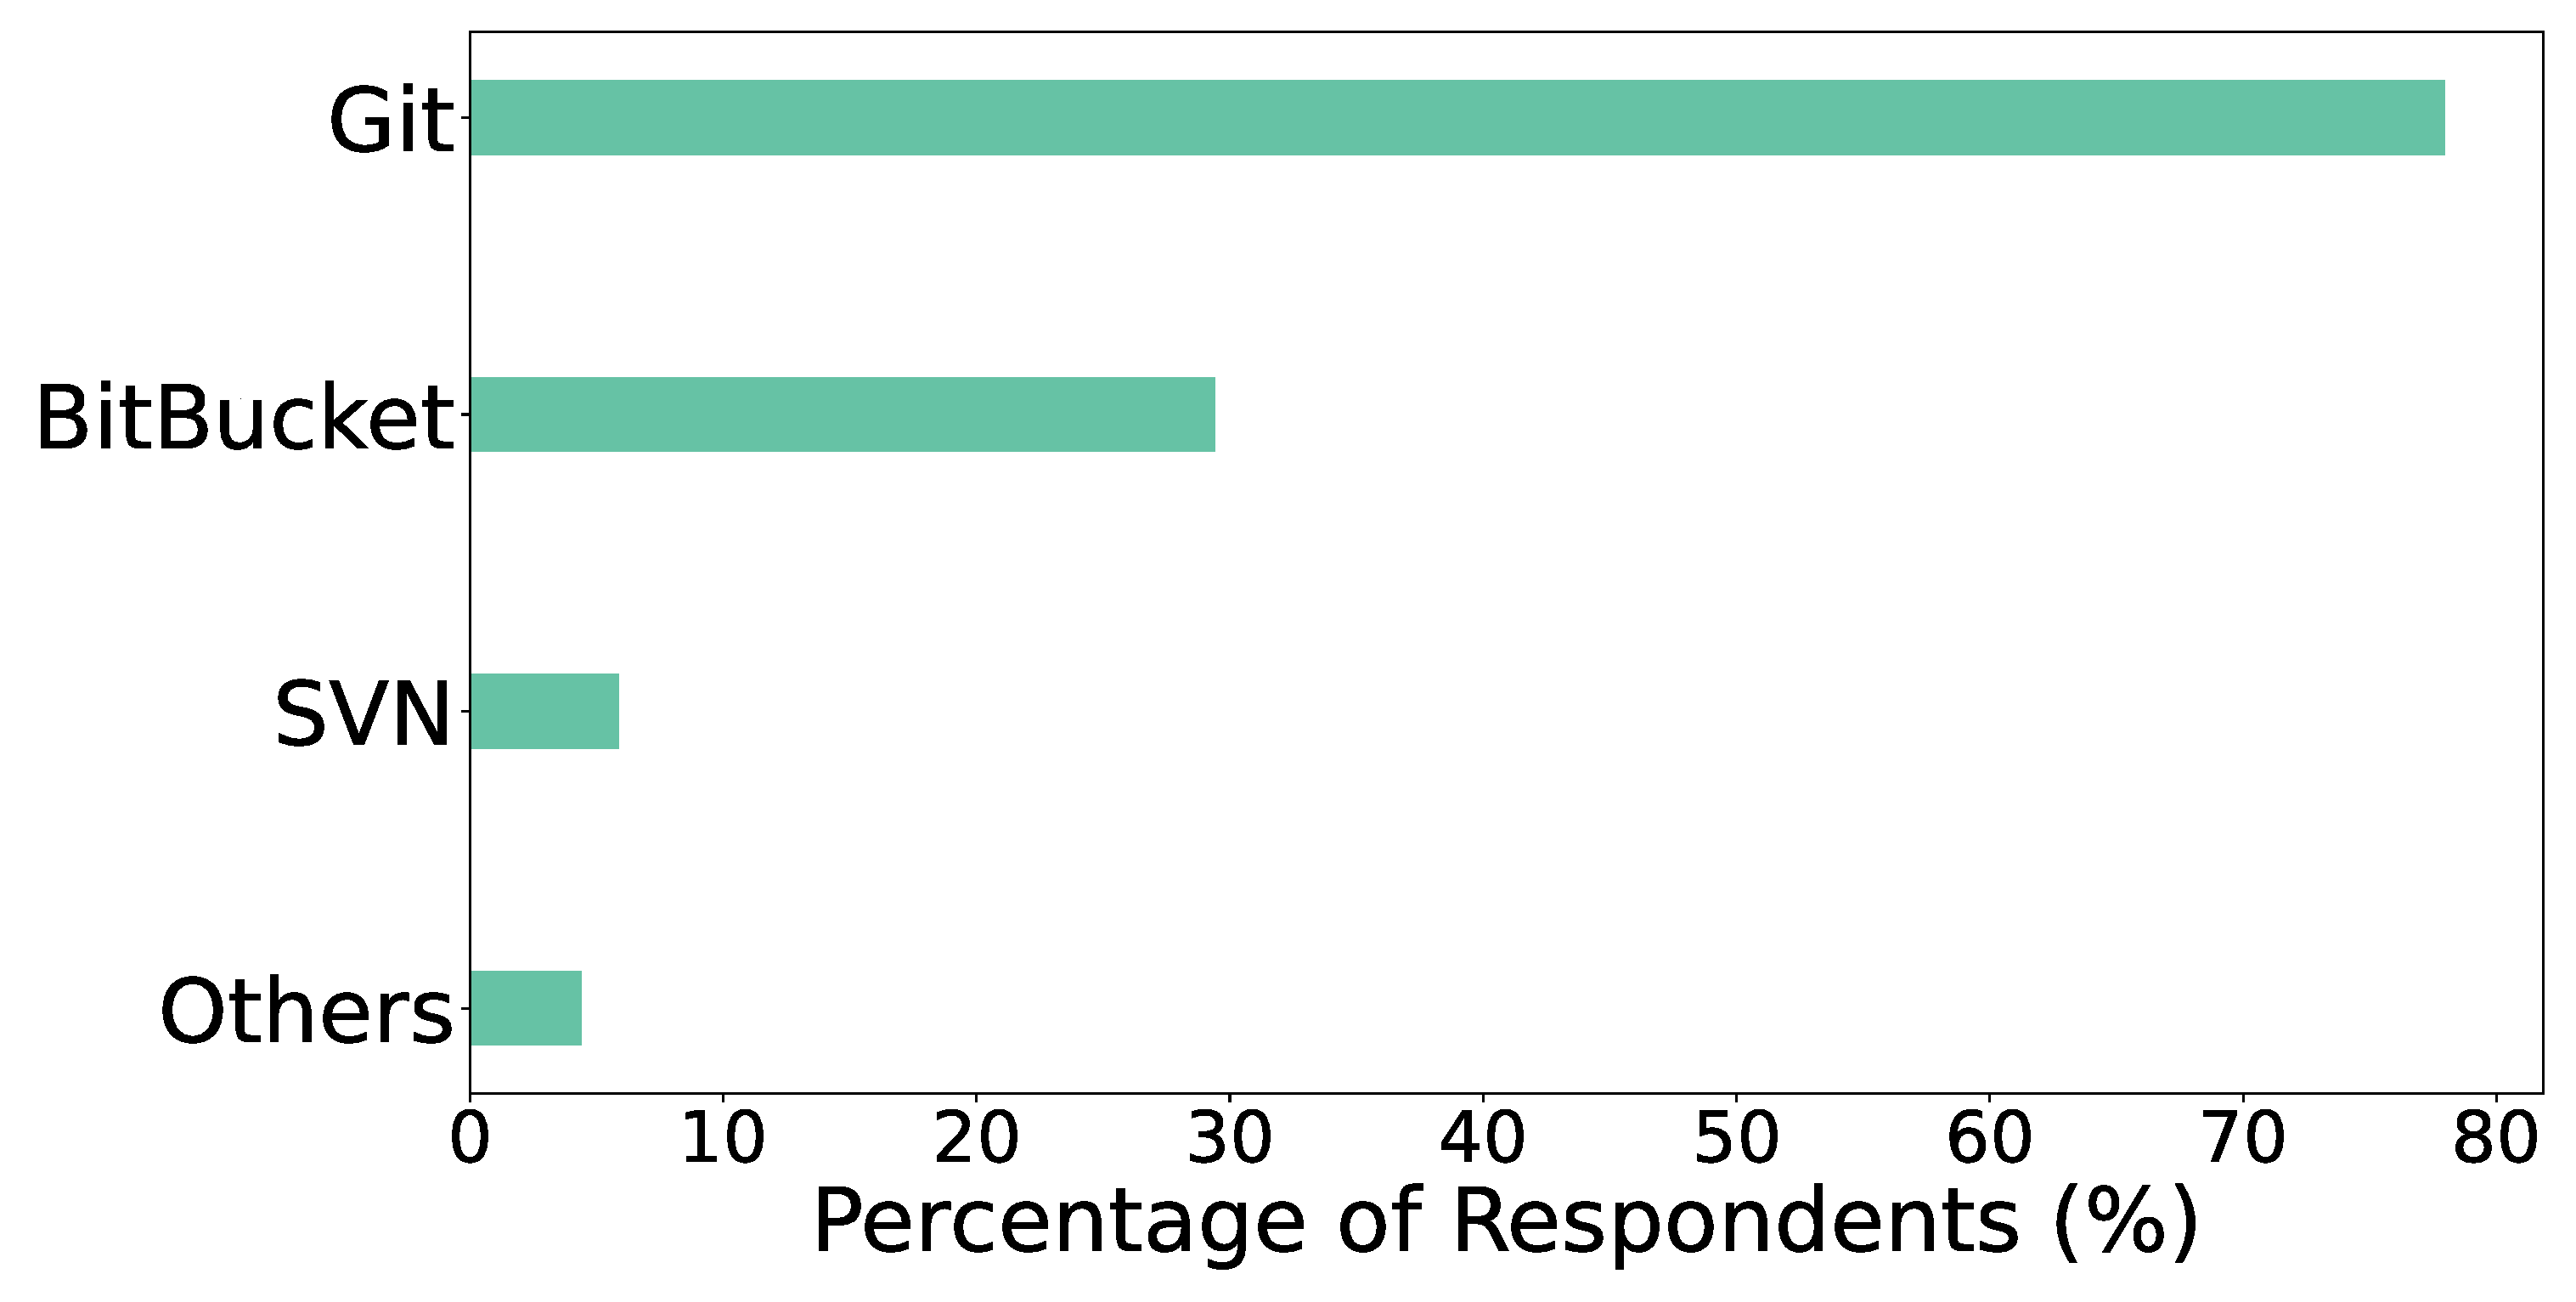
\includegraphics[scale=0.12]{Figures/Respondents_version_control}
        \caption{Version Control (Q18)}
        \label{fig:versionControl}
    \end{subfigure}
\end{figure}

% \begin{figure}[h]
% \centering
%   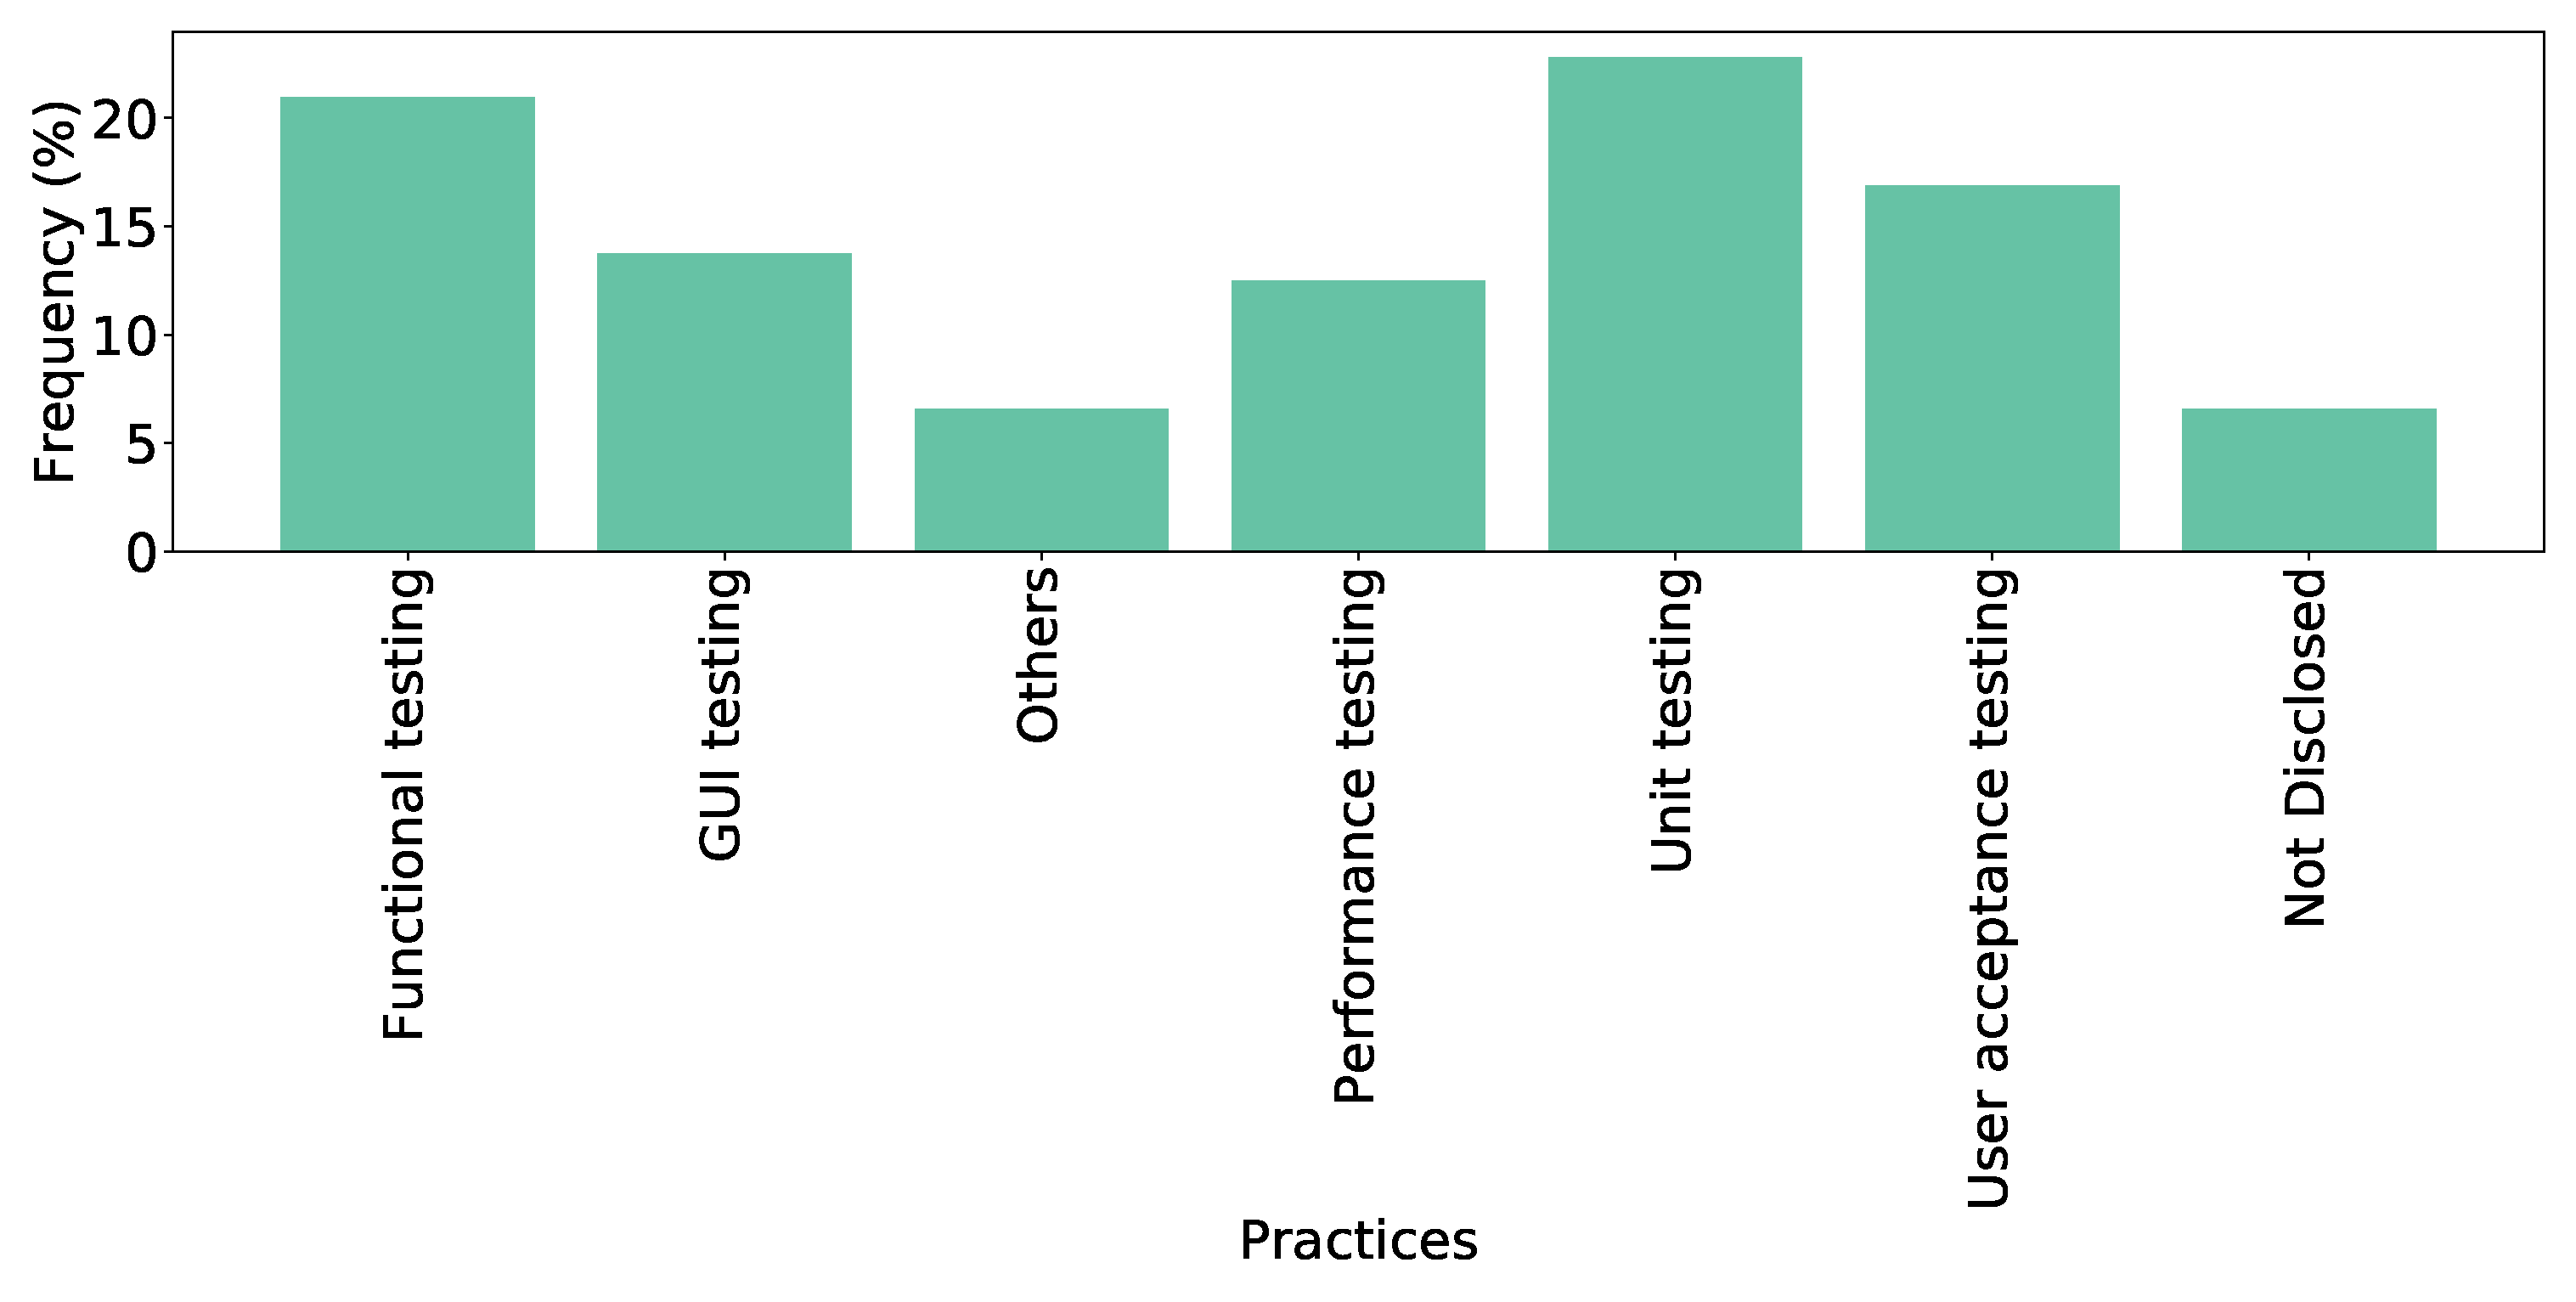
\includegraphics[scale=0.2]{Figures/Respondents_testing_practices}
%   \caption{Software Testing Practices (Q14)}
%   \label{fig:testing}
% \end{figure}
\nd\bf{$\bullet$ Software Testing Practices (Q14)}. According to Figure \ref{fig:testing}, several testing practices are used during
software development. The results show that most of the organizations have
carried out unit testing (53\%), functional testing (49\%), user acceptance
testing (39\%), GUI testing (31\%), etc. Unit testing also ranked first in the
2019 survey of JetBrains, where it was voted by 71\% participants across the
globe \citep{JetBrains2019}. We observed in our survey that in some cases
managers have reported performing GUI testing and performance testing, which is
unlikely in their role/designation. However, the observation is not
statistically significant ($p=0.12$). It may be deduced that in absence of
enough specialized resource managers have to take additional responsibility. To
identify the relation between testing practices and experience, we plotted them
together in Figure \ref{fig:testing type and experience}. We have observed that
junior developers (less than 5 years of experience) mostly perform unit, integration, and functional testing,
whereas senior developers mostly perform API testing. We conducted the Mann
Whitney U test to assess the conjecture, and it is found statistically
significant ($p<0.01$).

\begin{figure}[h]
\centering
  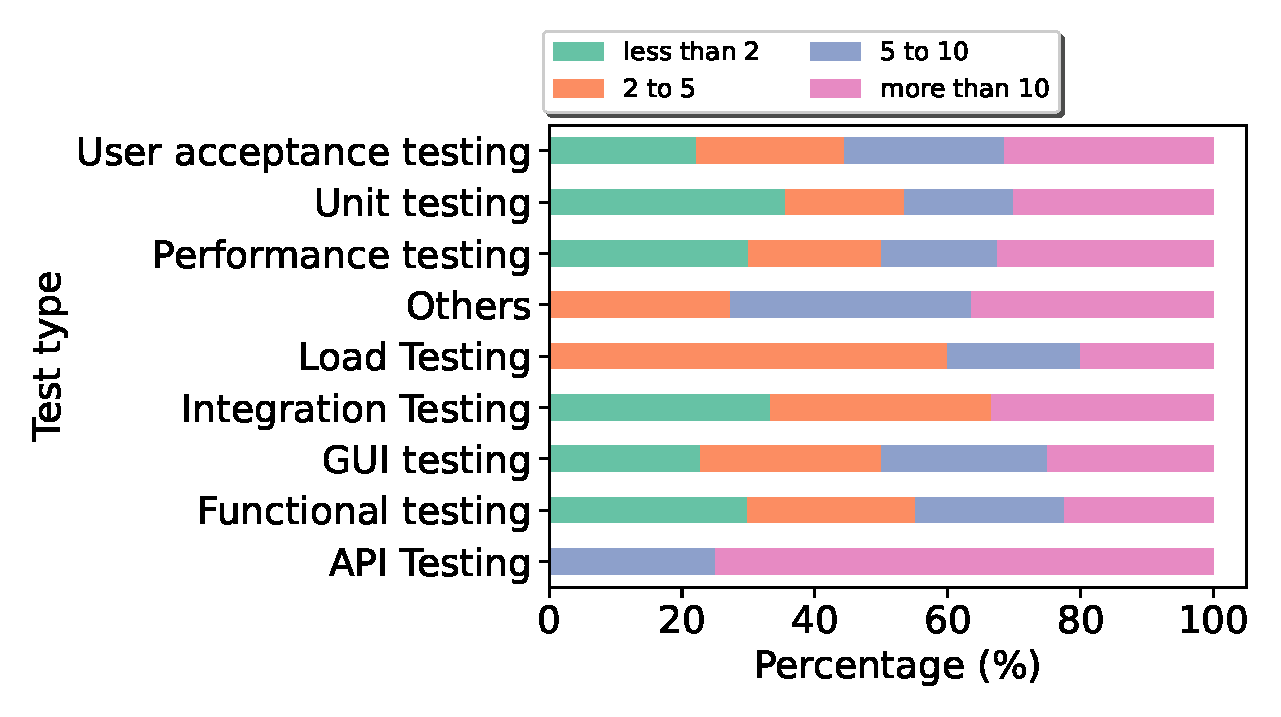
\includegraphics[scale=0.45]{Figures/Testing_Type_and_Experience}
  \caption{Testing practices ans professional experience}
  \label{fig:testing type and experience}
\end{figure}

% \begin{figure}[h]
% \centering
%   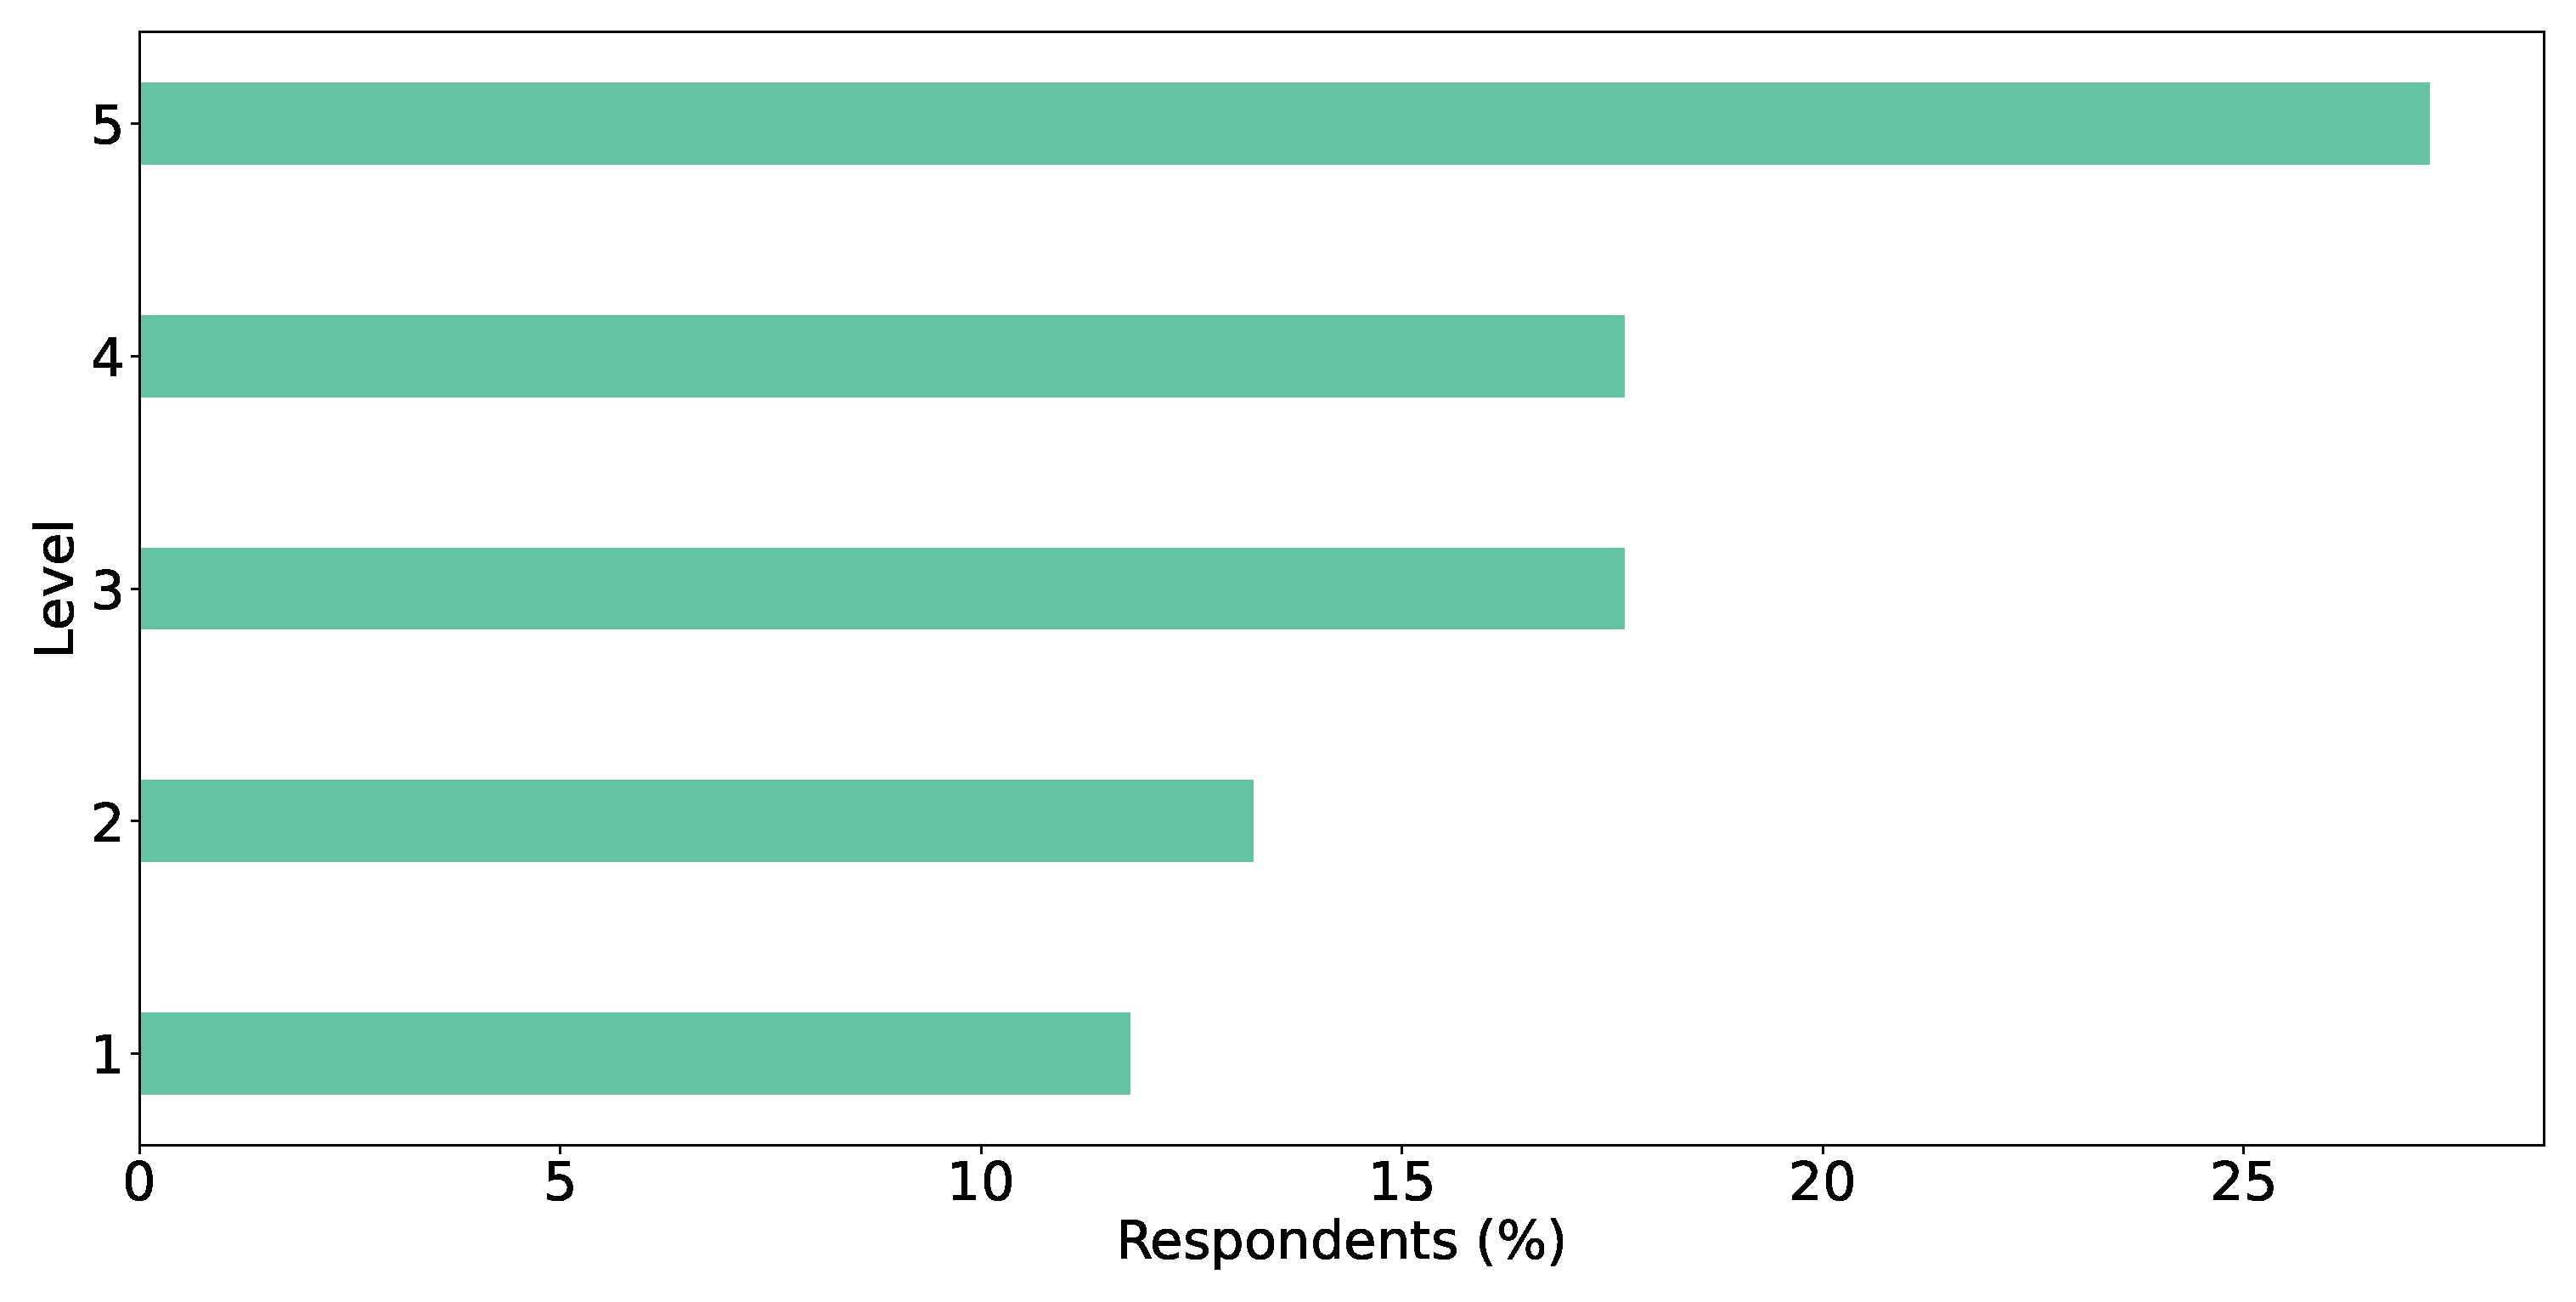
\includegraphics[scale=0.15]{Figures/Respondents_autotest_level}
%   \caption{Level of Automated Testing (Q15)}
%   \label{fig:autoTest}
% \end{figure}

\begin{figure}[t]
    \centering
    \caption{Analysis of automated testing level}
    \begin{subfigure}{0.5\textwidth}
        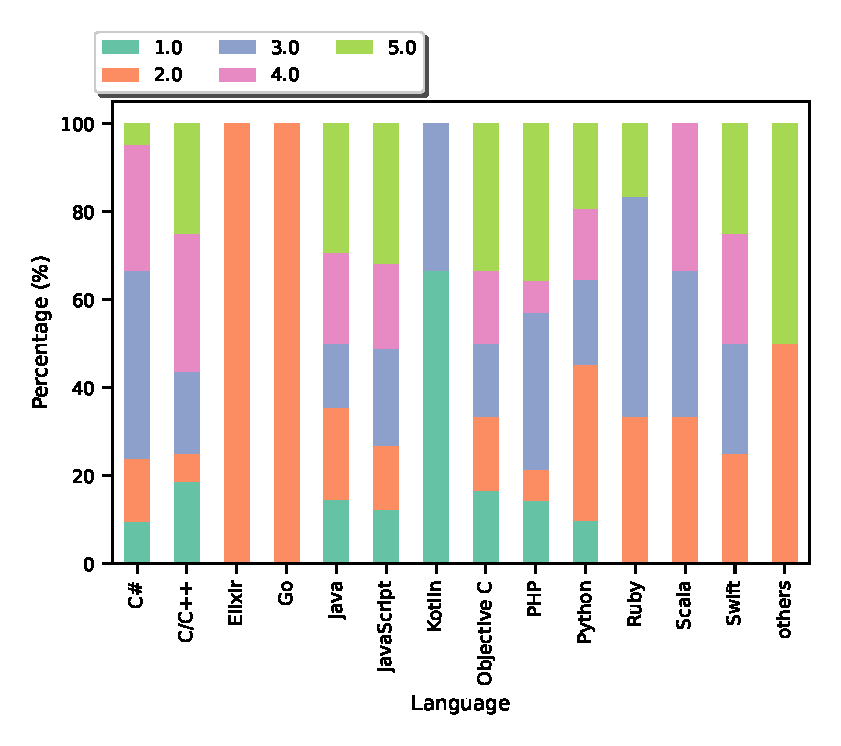
\includegraphics[scale=0.4]{Figures/Language_and_Test_Level}
          \caption{Programming language and automated testing level}
          \label{fig:language and autotest}
    \end{subfigure}
    \begin{subfigure}{0.4\textwidth}
          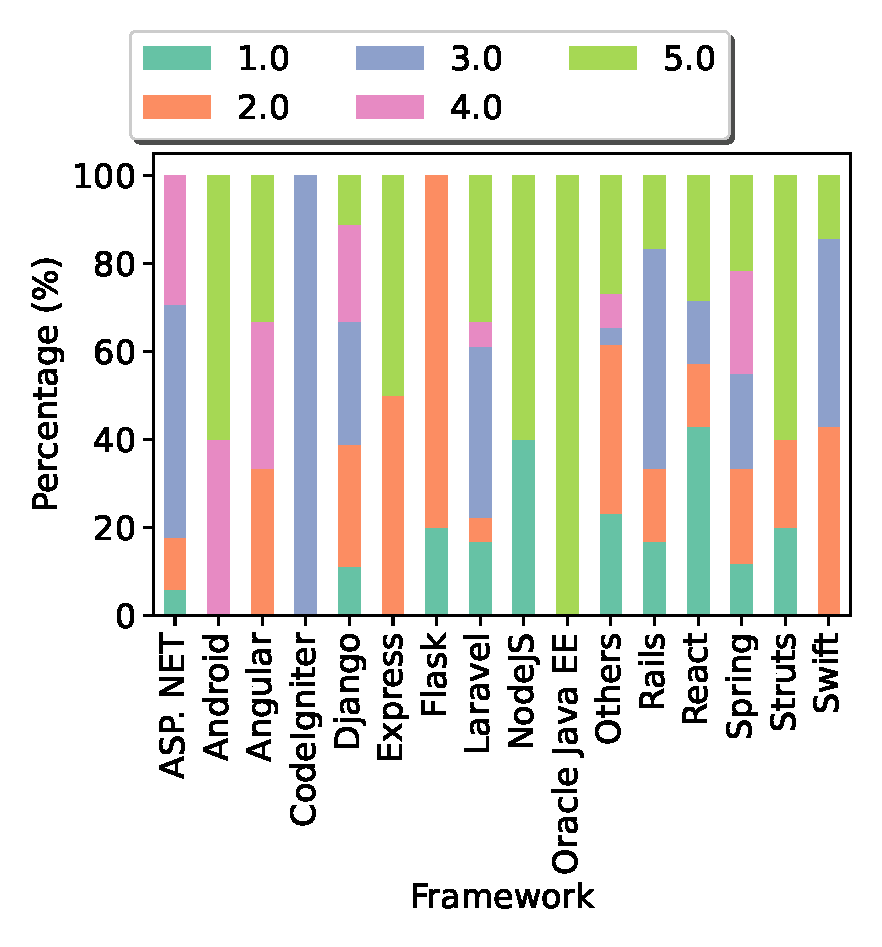
\includegraphics[scale=0.4]{Figures/Framework_and_Test_Level}
          \caption{Framework and automated testing level}
          \label{fig:framework and autotest}
    \end{subfigure}
\end{figure}

% \begin{figure}[h]
% \centering
%   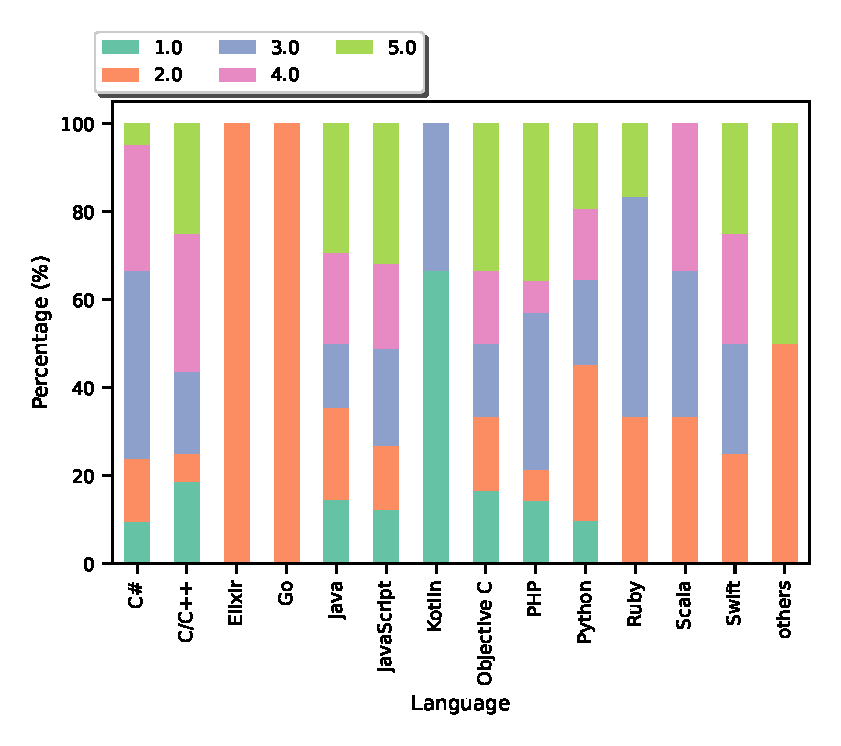
\includegraphics[scale=0.65]{Figures/Language_and_Test_Level}
%   \caption{Programming language and automated testing level}
%   \label{fig:language and autotest}
% \end{figure}

% \begin{figure}[h]
% \centering
%   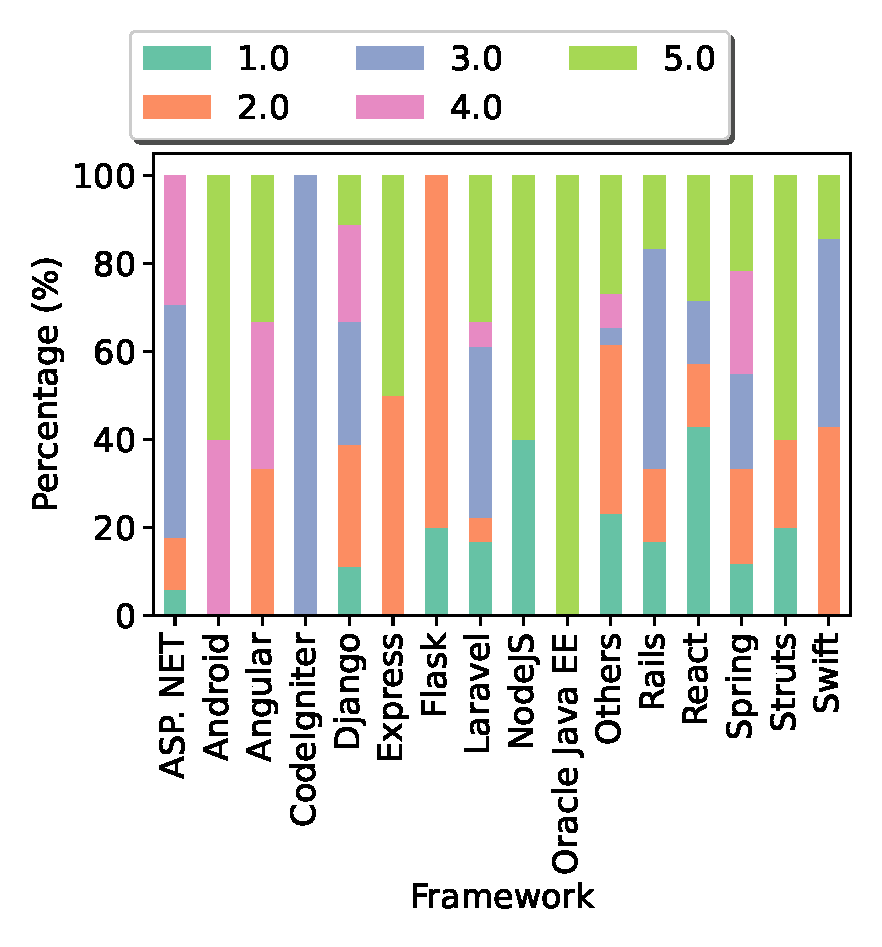
\includegraphics[scale=0.65]{Figures/Framework_and_Test_Level}
%   \caption{Framework and automated testing level}
%   \label{fig:framework and autotest}
% \end{figure}

% \begin{figure}[h]
% \centering
%   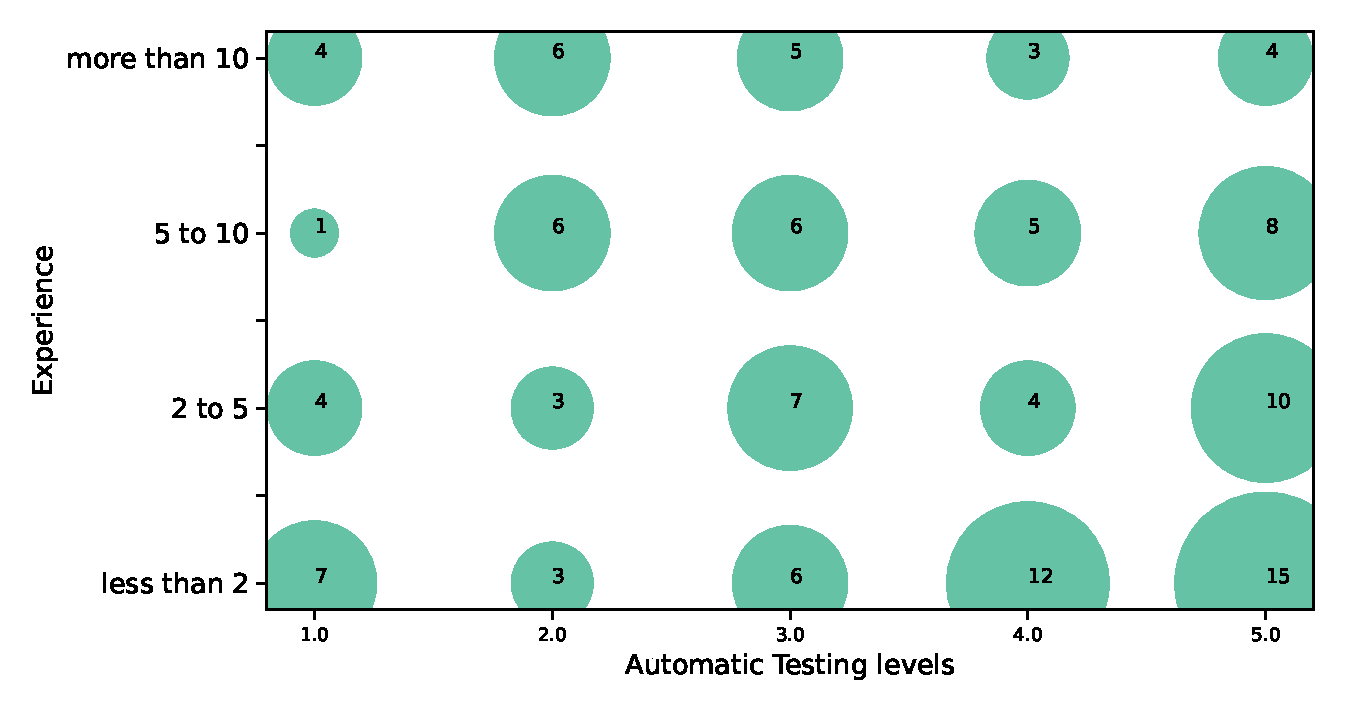
\includegraphics[scale=0.45]{Figures/Auto_Test_and_Experience}
%   \caption{Experience and automated testing level}
%   \label{fig:experience and autotest}
% \end{figure}
\nd\bf{$\bullet$ Level of Automated Testing (Q15).}
We have asked the survey participants about the level of automated testing
performed in their respective companies. The responses were gathered using the
Likert scale. It was found that different respondents have very different
experiences in this context, i.e., some companies heavily practice automated
testing, while others favor manual testing. 
Results are shown in Figure
\ref{fig:autoTest}, which indicates that about 70\% of our respondents (others
than who voted for level 5) do not use automated testing regularly. The level of
automated testing might be related to the programming language/framework. The
testing suite provided by framework/language might encourage developers to
implement automated testing. The level of automated testing vs. language and
framework is plotted in Figures \ref{fig:language and autotest} and
\ref{fig:framework and autotest}, respectively. It seems from Figure
\ref{fig:language and autotest} that the highest level of automated testing is
mostly practiced in Java, JavaScript, Objective-C, and PHP language. We
conducted the Mann Whitney U test to assess our conjecture and it is found
statistically significant ($p=0.01$). From Figure \ref{fig:framework and
autotest}, we found that the highest level of automated testing is mostly
performed in Android, Express, Node.js, Struts, and Java EE framework, and the
observation is statistically significant ($p=0.006$). Also, the highest level of
automated testing is mainly used by developers (unit testing). 
Managers practice the lowest level of automated testing. We observed that managers mainly engaged in assessing the
acceptability of the product from the end-user point of view. We also observed that Junior developers tend to use more automated testing than senior
developers. However, the observation is not statistically significant
($p=0.08$). One reason behind this observation may be that the senior
developers perform GUI testing more, which are hard to
automate.


% \begin{figure}[h]
% \centering
%   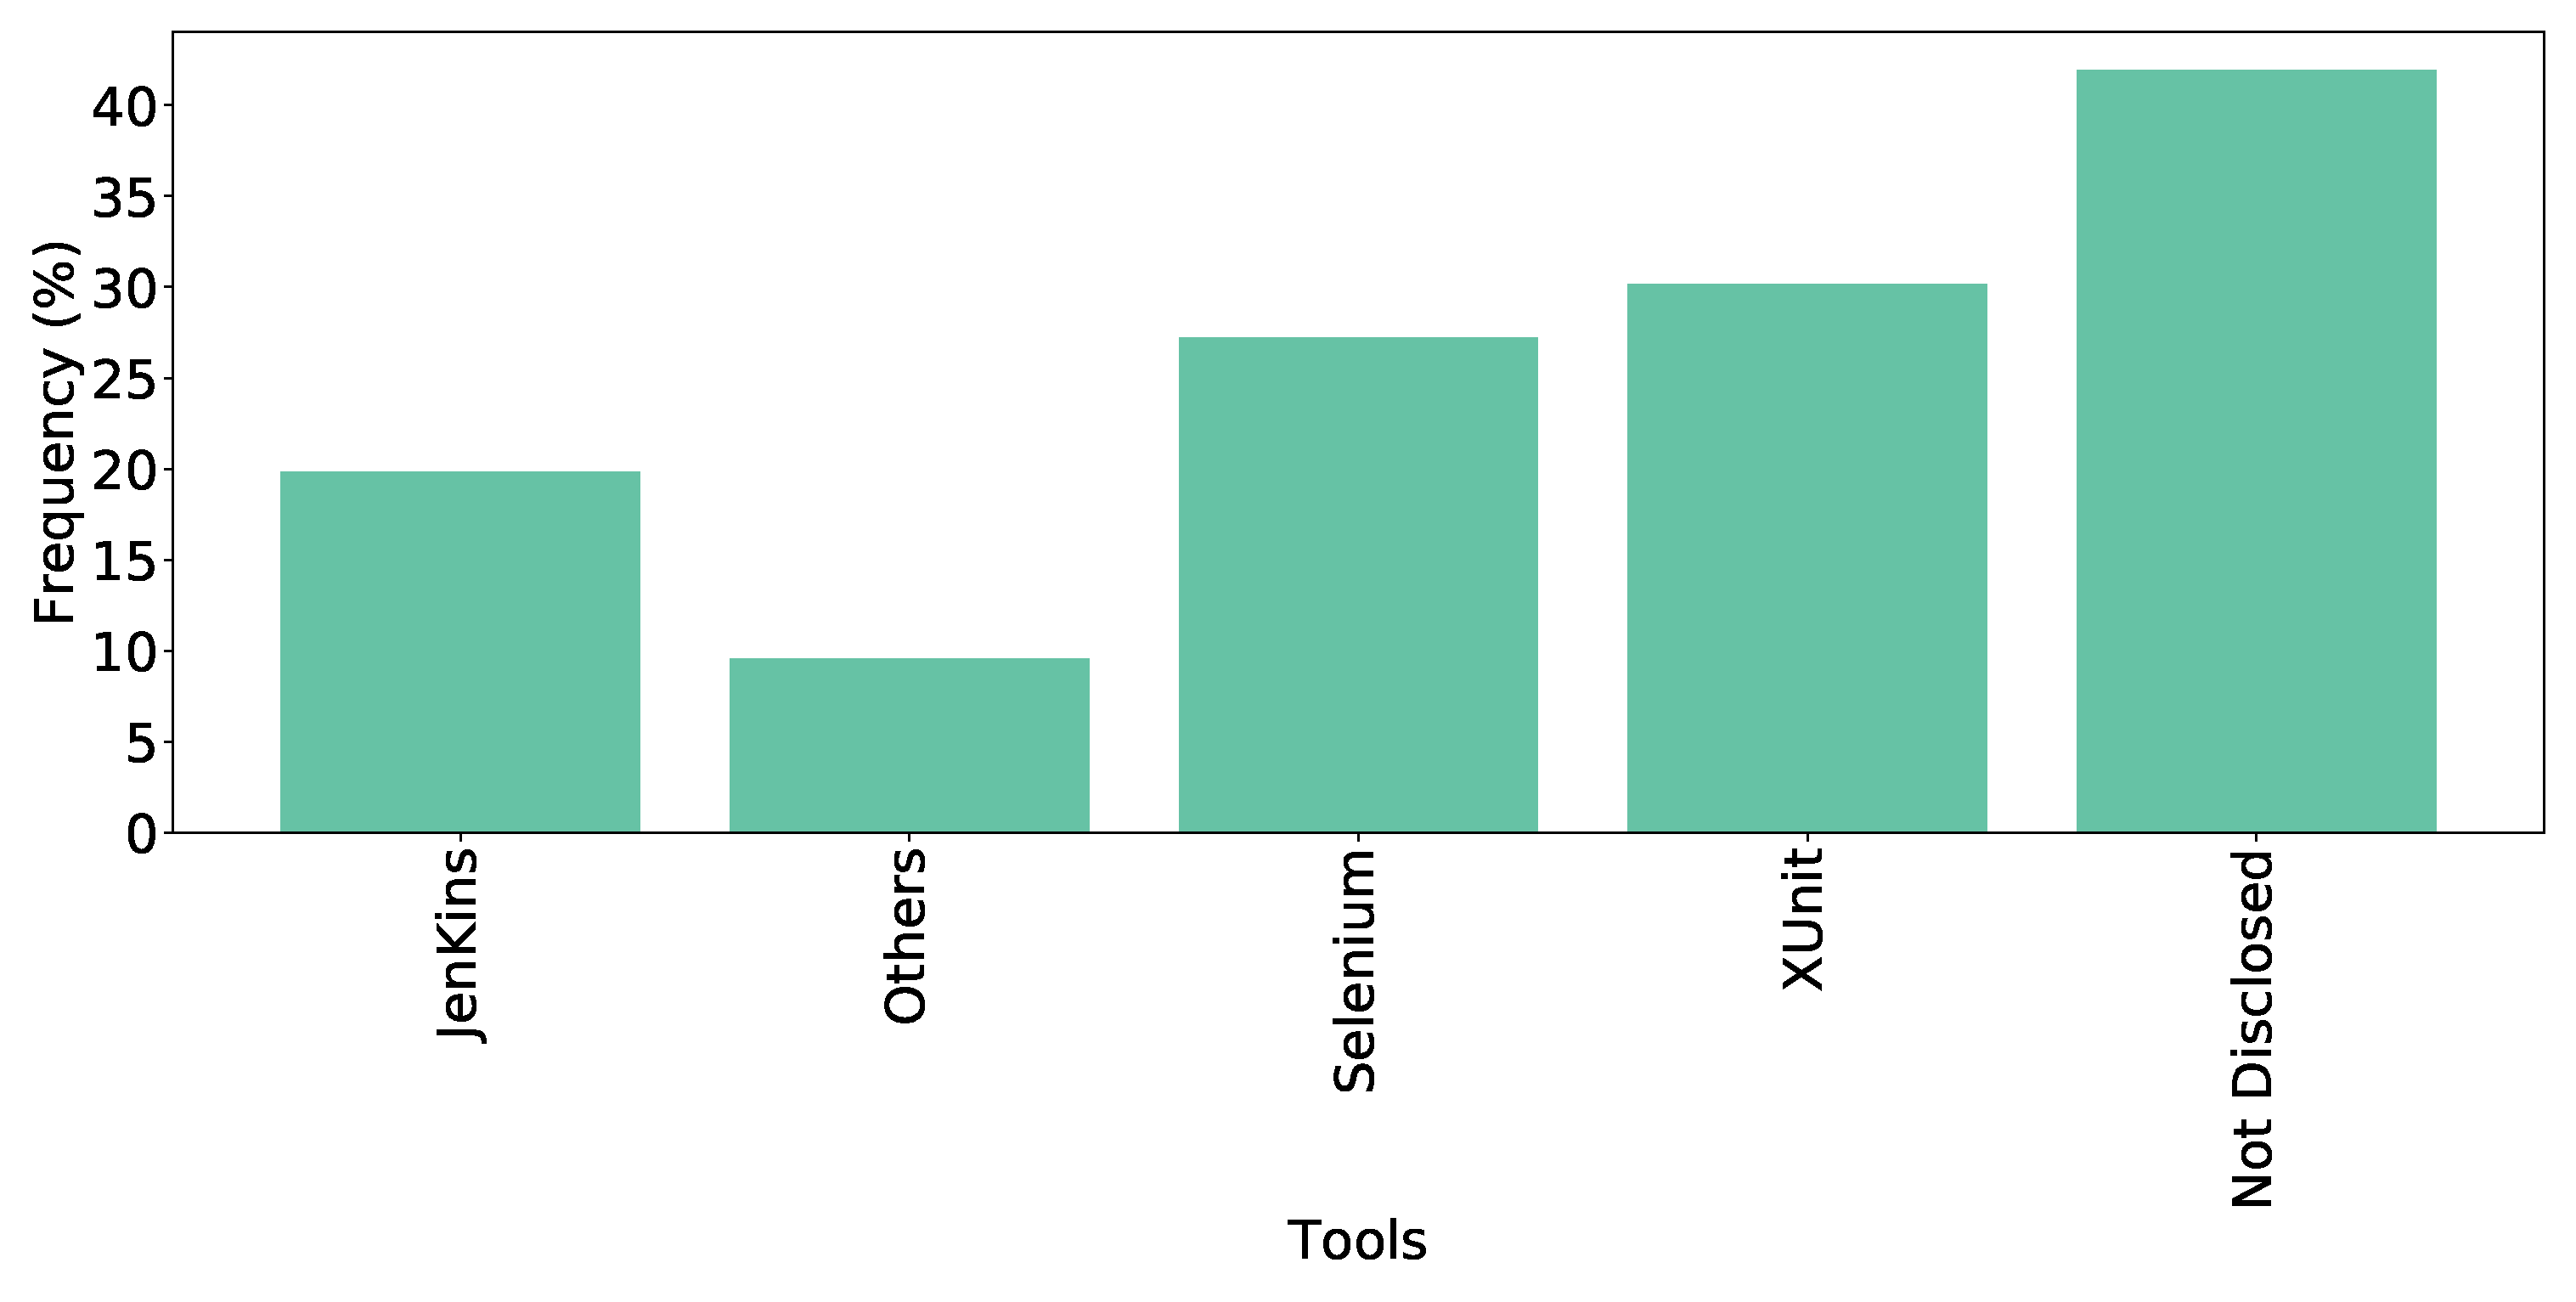
\includegraphics[scale=0.18]{Figures/Respondents_testing_tools}
%   \caption{Tools Used in Testing and QA (Q16)}
%   \label{fig:testingTools}
% \end{figure}
\nd\bf{$\bullet$ Tools Used in Testing and QA (Q16).} Most of the
respondents have used XUnit (e.g., JUnit, NUnit) (30\%), Selenium (27\%),
Jenkins (20\%), others (9\%) (see Figure \ref{fig:testingTools}). Around
38\% of our respondents were not interested in replying to this question that is
not surprising because the majority of the respondents (93\% approx.) were
working on roles other than SQA engineer as per Table \ref{tab:role}, and they
are not supposed to be involved in any testing themselves. 
%\anindya{This may be
%because many developers are not involved in any sort of testing themselves and
%our respondents are dominated by developers.} \khalid{updated}

%\boxtext{There has a large demand of software testing tools in Bangladesh.}

% \begin{figure}[h]
% \centering
%   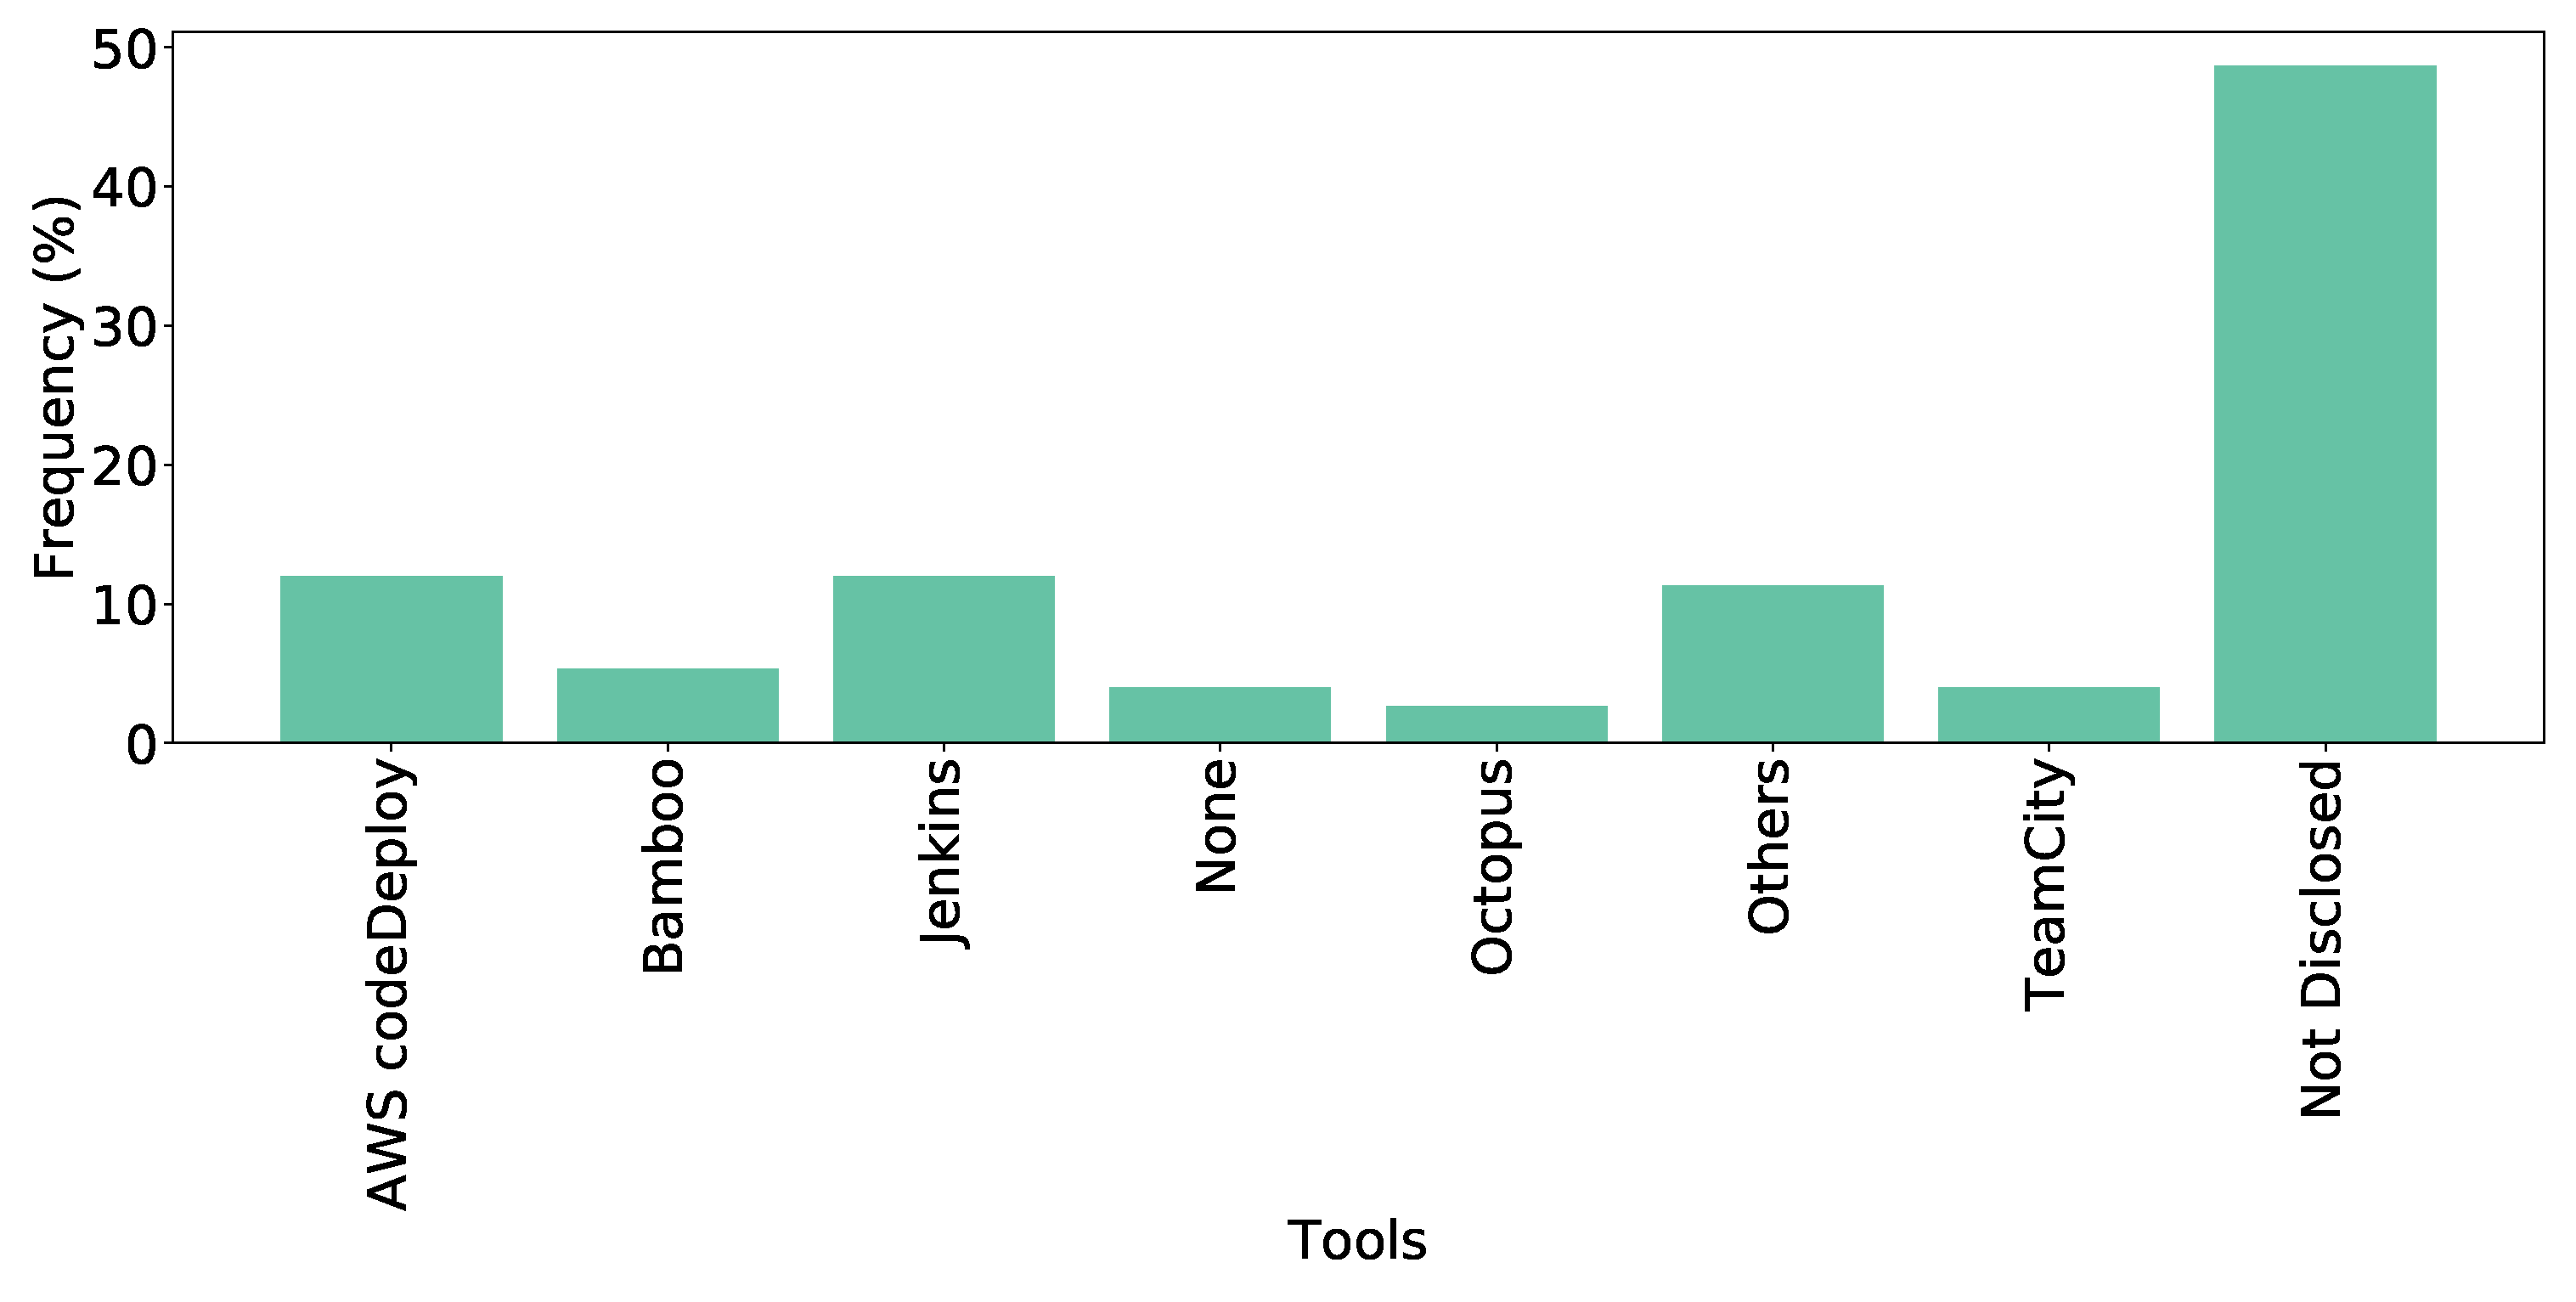
\includegraphics[scale=0.18]{Figures/Respondents_deployment_tools}
%   \caption{Continuous Deployment tools (Q17)}
%   \label{fig:deployTools}
% \end{figure}

\nd\bf{$\bullet$ Continuous Deployment tools (Q17).} majority of the respondents deploy their implemented codes using AWS code-deploy
(12\%) and Jenkins (12\%) (Figure \ref{fig:deployTools}). The other deployment tools are Bamboo (5\%), TeamCity
(4\%), Octopus (2\%), etc. Respondents voted none (4\%) as they didn't use any
deployment tools and 53\% of the respondents were not interested in this topic.
Anyhow, the percentage of uninterested respondents does not seem unexpected.
From Table \ref{tab:role} and \ref{tab:experience}, we can observe that a
significant portion of our respondents is developers, and more than half of our
respondents are experienced for less than five years respectively. As deployment
is related to DevOps, it is quite likely that developers have not enough
knowledge or have less interest in deployment. 
%\anindya{Again, this is mostly a
%dev op related issue and the developers are not likely to respond in this
%regard.} \khalid{updated} 
The outcome indicates that the usage rate of
deployment tools in Bangladesh for continuous integration and continuous
deployment is not widespread yet. 
%We also guessed that the practice of using
%deployment tools might be done only by senior practitioners. However, the
%hypothesis is not statistically significant ($p=0.37$).
%\rifat{We are saying implicitly that the survey is for developers, not for QA and DevOps engineers. Is it OK?}

% \begin{figure}[h]
% \centering
%   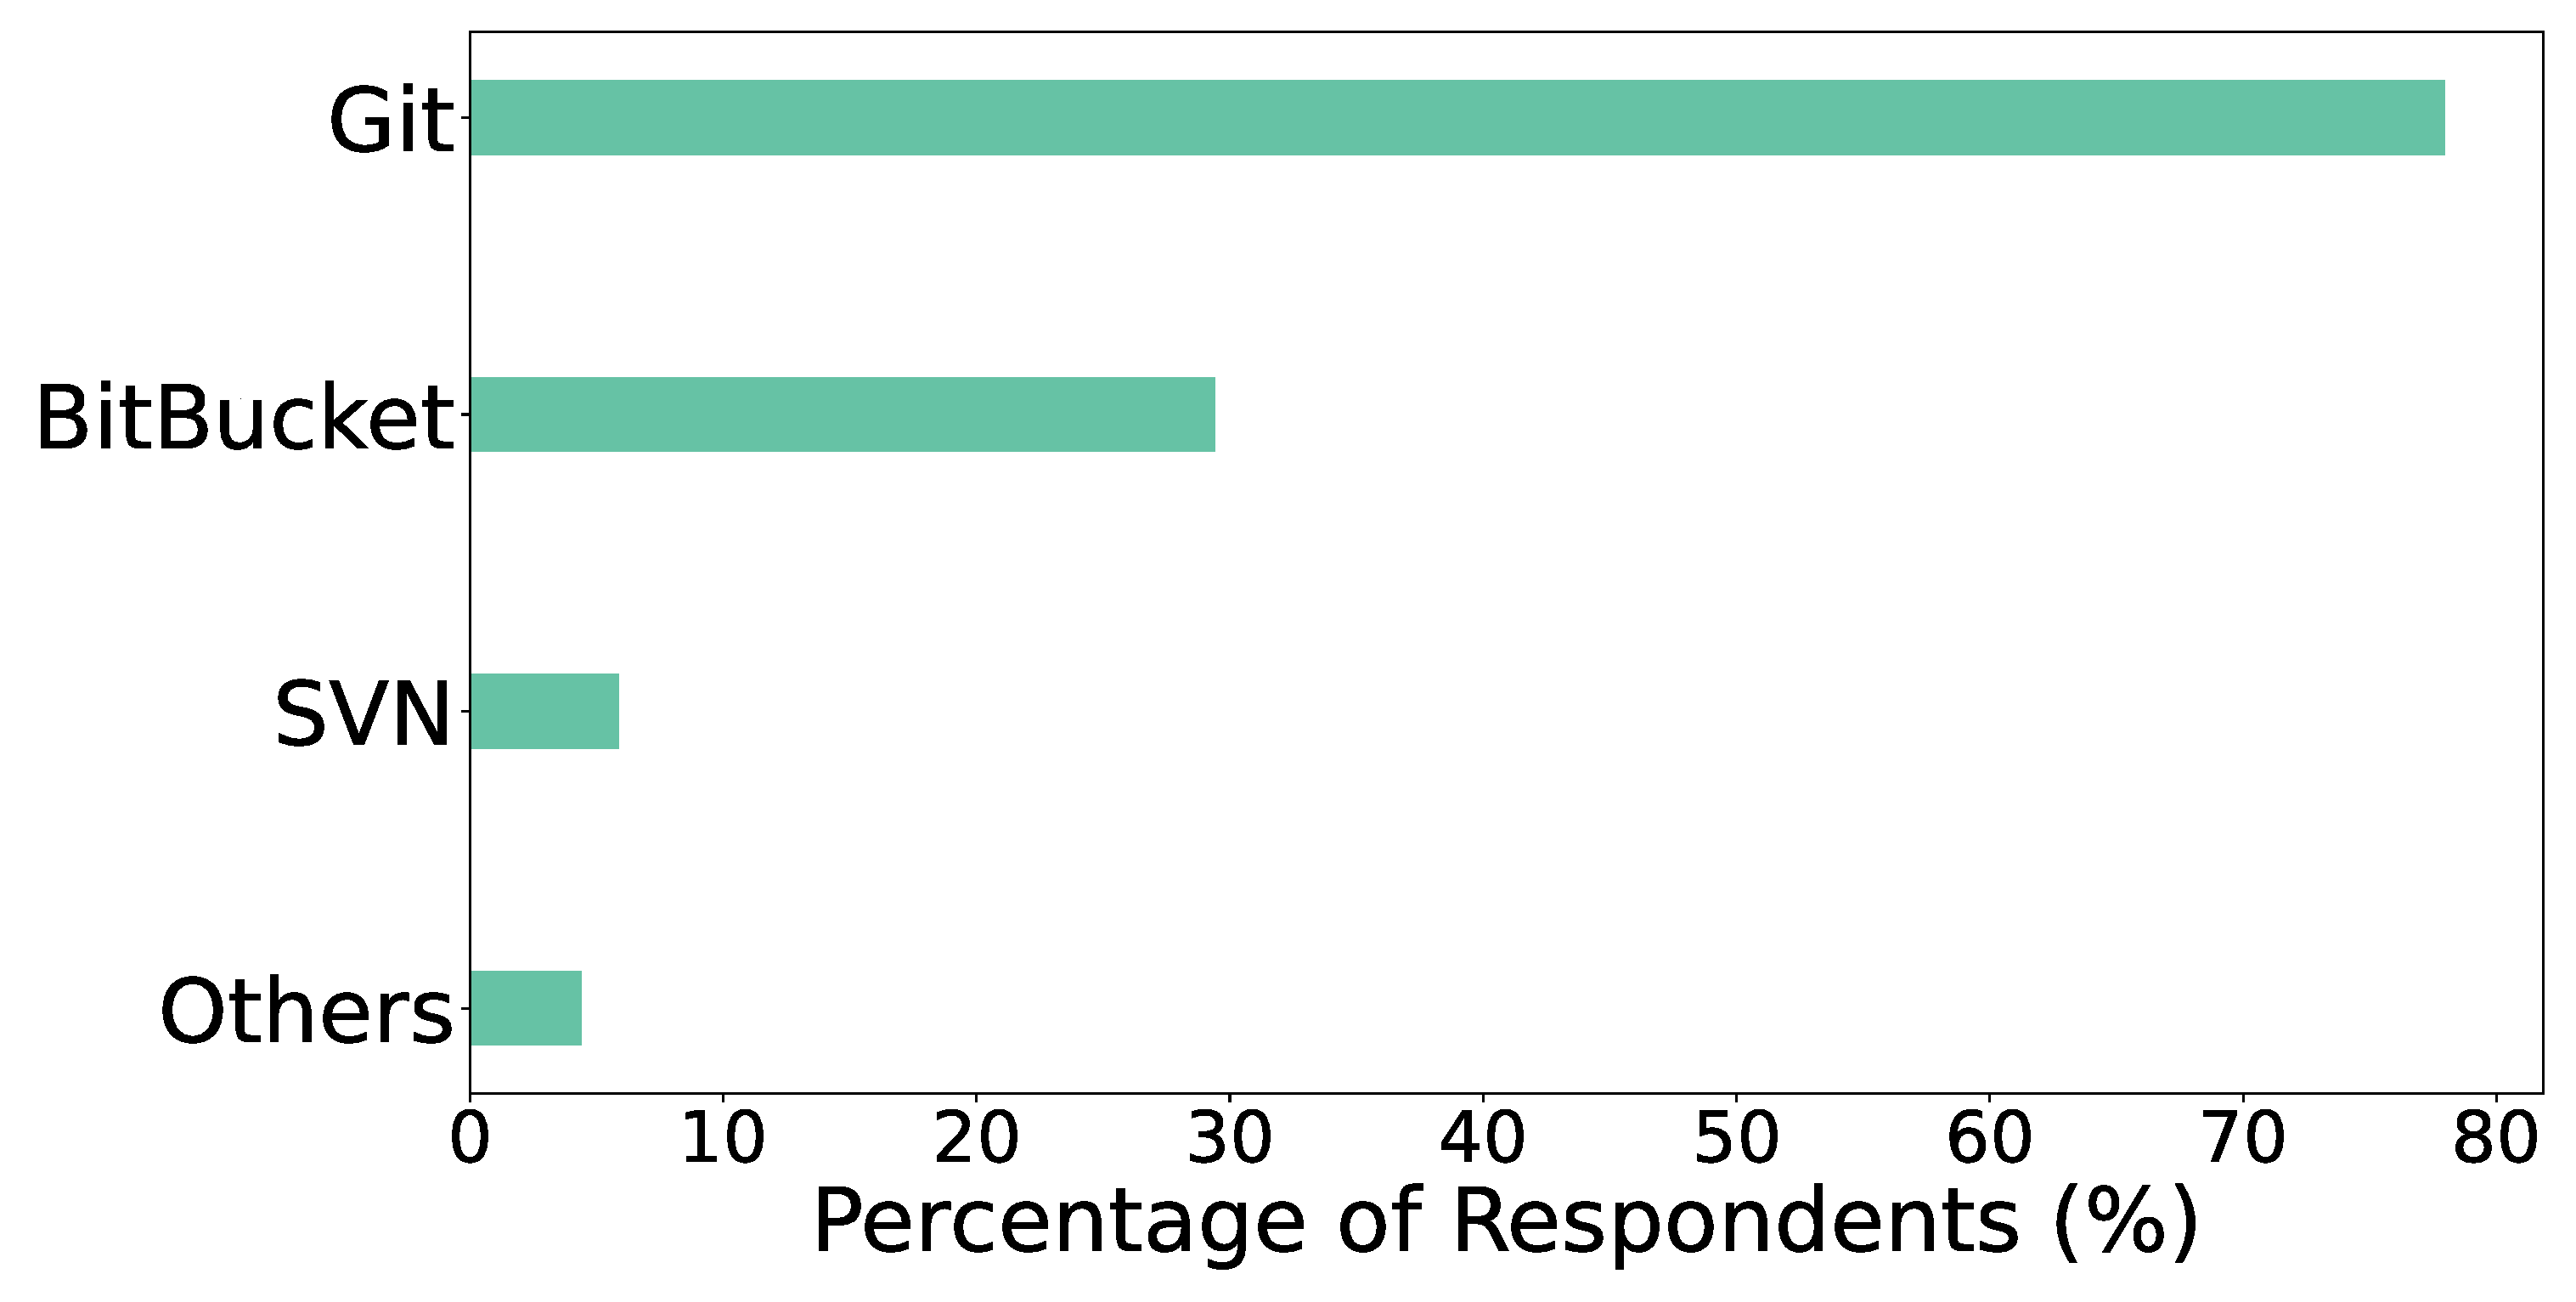
\includegraphics[scale=0.16]{Figures/Respondents_version_control}
%   \caption{Version Control (Q18)}
%   \label{fig:versionControl}
% \end{figure}
\nd\bf{$\bullet$ Version Control (Q18).} Git (78\%) and Bitbucket (29\%) are mostly-used
version control systems in the software industry.% as shown in Figure \ref{fig:versionControl}. 
 Besides these, Subversion (SVN) (5\%) and others (4\%)
are used.  Respondents were allowed to select more than one option. The 2018
Stack overflow survey\citep{StackoverflowSurvey2018} reports that the most
popular version control system is Git (87.2\% developer uses Git) and the second
most popular is SVN (16.1\% developer uses SVN). However, in our survey, we
found a slightly different result, the most popular version control system is
Git and the second most popular is Bitbucket. This might be related to the
declining popularity of SVN over the years. From the Stack overflow survey over
the range 2017-2018, it is clear that SVN is losing popularity to Git. 
%Nowadays,
%SVN is mainly used for versioning legacy projects. As the SE industry of
%Bangladesh is relatively young, this discrepancy observed is not surprising.
% \anindya{It looks nice that you compared with external relevant source like SO. Is it possible to do it for other RQs? Also, you may mention such deviations from other trends in Introduction.} \khalid{added in `methodologies', `tech platform', `test practices'} \partha{added in `os', `languages', `framework'}

\begin{tcolorbox}[flushleft upper,boxrule=1pt,arc=0pt,left=0pt,right=0pt,top=0pt,bottom=0pt,colback=white,after=\ignorespacesafterend\par\noindent]
\nd\it{\bf{RQ1-D3. Software testing and devops practices used.}} Unit testing is
heavily carried out by developers in the Bangladesh SE industry likewise across
the globe. In addition, various software testing
tools (e.g., XUnit, Selenium, etc.) and deployment tools (e.g., AWS code-deploy,
Jenkins, etc.) are used. However, there is a tendency among most
Bangladeshi developers not to use these automated tools regularly. 
Git is the most popular version control system, while SVN is losing
its popularity in the Bangladesh SE industry likewise across the globe.
%\gias{summarize RQ1-D3 here} \khalid{updated}
\end{tcolorbox}
